\documentclass[12pt,english]{article}

\usepackage[utf8]{inputenc}
\usepackage[T1]{fontenc}
\usepackage[a4paper]{geometry}
\geometry{verbose,tmargin=1.5cm,bmargin=2.5cm,lmargin=2.8cm,rmargin=2cm}
\usepackage{verbatim}
\usepackage{algorithm}
\usepackage{algpseudocode} % modern replacement for 'algorithmic'
\usepackage{amsmath}
\usepackage{amssymb}
\usepackage{amsfonts}
\usepackage{array}
\usepackage[main=english,greek]{babel}
\usepackage{csquotes}
\usepackage[backend=biber, style=numeric-comp, sorting=none]{biblatex}
\usepackage{booktabs}
\usepackage{colortbl}
\usepackage{enumitem}
\usepackage[T1]{fontenc}
\usepackage{graphicx}
\usepackage{hyperref}
\usepackage{listingsutf8}
\usepackage{listings}
\usepackage{multirow}
\usepackage{physics}
\usepackage{textgreek}
\usepackage[table,xcdraw]{xcolor}
\usepackage{tikz}
\usetikzlibrary{shapes.geometric, arrows.meta, positioning}
\usepackage{lmodern}

\newtheorem{definition}{Definition}[section]

\addbibresource{fsm.bib}
\lstset{basicstyle=\ttfamily}
\lstset{inputencoding=utf8/latin1}

% Adjust tables row height
\renewcommand{\arraystretch}{1.5}
% Make COMMENT truly inline, no line break
\newcommand{\InlineComment}[1]{\quad\texttt{// #1}}

\begin{document}
% \title{A novel discrete toy universe}
\title{It from bit: a concrete attempt}
\author{Alexandre Furtado Neto \\ UNESP Alumnus \thanks{alexandre.com@yahoo.com, ORCID 0000-0001-9435-6566.}}
\maketitle

\begin{abstract}
This work proposes a toy universe model based on classical logic, elementary arithmetic, and a hint of topology, using a discrete, finite 3-torus structure with an additional non-spatial dimension. Each point in this space holds a binary string with ontological significance, evolving through simple rules to produce complex patterns, including spherical propagation and harmonic behavior. We explore how these dynamics emulate fundamental physical phenomena, offering a novel framework for digital physics.  It is not intended as an interpretation of Quantum Mechanics but rather as an attempt to describe nature at a more fundamental level.

\medskip{}
\end{abstract}

\vfill

\begin{center}
\textbf{PACS numbers: }12.10.Kt, 03.65.Ta, 04.60.Pp, 05.45.-a
\par\end{center}

\begin{center}
\textbf{Keywords}: cellular automaton, non-locality, emerging gravity, unification, magnetic monopole
\par\end{center}

\newpage

%%%%%%%% INTRODUCTION %%%%%%%%%%

\section{Introduction}

John Archibald Wheeler's aphorism ``it from bit'' encapsulates a profound idea: the physical world, at its most fundamental level, may emerge from discrete binary choices, or bits, suggesting that information is the bedrock of reality \cite{wheeler}. This perspective, central to the field of digital physics, posits that physical phenomena, including those described by quantum mechanics and general relativity, could arise from computational processes governed by simple rules. Cellular automata (CA), mathematical models of discrete space and time evolving through local rules, offer a natural framework for exploring this idea, as their simplicity can give rise to complex, emergent behaviors reminiscent of physical systems \cite{wolfram,zuse,fredkin}.

This work introduces a novel toy universe model grounded in classical logic, elementary arithmetic, and topological principles, designed to explore how fundamental physical phenomena might emerge from a deterministic CA framework. Unlike traditional interpretations of quantum mechanics, which rely on probabilistic descriptions, our model seeks to describe nature at a deeper, ontological level, where particles, forces, and spacetime emerge from the interactions of binary states in a finite, discrete structure. Specifically, we propose a universe defined on a 3-torus topology with a non-spatial dimension, where each point contains a fixed-size bit string encoding ontological properties. These bit strings evolve through local rules, producing patterns such as spherical wavefronts, harmonic oscillations, and symmetry-breaking patterns, which we map to physical analogs like particles, electromagnetic interactions, and gravitational effects.

Our approach builds on foundational work in digital physics, including Konrad Zuse’s pioneering CA-based universe model \cite{zuse}, Edward Fredkin’s reversible computing framework \cite{fredkin}, and Stephen Wolfram’s exploration of complex behavior from simple rules \cite{wolfram}. However, we diverge by introducing a layered 3-torus structure and specific interaction rules that emulate quantum-like and relativistic phenomena without invoking probabilistic superpositions. This model is not intended as a direct interpretation of quantum mechanics but as a speculative framework to probe whether a deterministic, information-based universe can reproduce observed physical phenomena.

The paper is organized as follows: Section \ref{sec:related-work} begins with a review of previous work in the area, followed by Section \ref{sec:space-and-time} with the foundational stage, defining the universal fabric. Section \ref{initial-state} builds the initial state. The light frame is presented in Section \ref{sec:light-frame}. Section \ref{sec:Particles} defines particles, followed by Section \ref{sec:Interactions} that illustrates bubble interactions and explores the role of charge conjugation. Section \ref{sec:Results} provides key results. Section \ref{sec:bridge} succinctly contemplates the bridge between the model and the QM formalism, and Section \ref{sec:Prospects-and-conjectures} outlines potential future directions. Finally, Section \ref{sec:Discussion} offers a summary and a synthetic interpretation of the model.

\section{Related work} \label{sec:related-work}

\subsection*{Stanislaw Ulam and John von Neumann}
Stanislaw Ulam, while working at Los Alamos in the 1940s, studied crystal growth using a simple lattice network, which laid some groundwork for the concept. He also suggested to John von Neumann the use of a discrete system for modeling self-replication \cite{ulam1952,vonNeumann1966}.

Inspired by Ulam's work and his own interest in self-replicating systems, von Neumann is considered the originator of cellular automata (CA) theory in the late 1940s and early 1950s. He developed a complex 29-state CA on a 2D grid to model self-replication. His work laid the foundation for much of the subsequent research.

\subsection*{Konrad Zuse}
Zuse proposed the first CA-based universe model~\cite{zuse}—the idea that the universe is a giant digital computation, laying the foundations of digital physics decades before it became a popular concept.

He suggested that space and time are discrete, and that physical processes are the result of local rule-based updates, echoing what we now call CA behavior. All of physics could emerge from information processing on a discrete grid of finite-state machines.

Zuse’s ideas inspired and legitimized later work in digital physics and CA-based universe models, influencing:

\subsection*{Edward Fredkin}
Fredkin \cite{fredkin} built upon Zuse’s vision with reversible computing. He was one of the earliest and most influential thinkers to propose that the entire universe might be a cellular automaton. His radical idea—often called digital physics or the Fredkin Finite Nature Hypothesis—suggests that reality evolves by discrete state changes, much like a cellular automaton. Space, time, and matter are all the result of information processing on a computational substrate. Everything is information.

Fredkin was a strong advocate of reversible computation, which preserves information—a key principle of both thermodynamics and quantum mechanics. He co-developed the Fredkin Gate, a reversible logic gate central to thinking about CA-based universes where no information is lost.

\textbf{Philosophical Implications:}
\begin{itemize}
  \item The universe is not just like a computer—it \emph{is} a computer.
  \item Particles are patterns of information, not physical substances.
  \item Physical laws may be \emph{emergent programs} running on a CA-like system.
\end{itemize}

Fredkin’s ideas deeply influenced Norman Margolus, Stephen Wolfram, and Konrad Zuse.

\subsection*{Martin Gardner}
M. Gardner popularized Conway’s Game of Life in \emph{Scientific American}, sparking widespread interest in CA and complex systems \cite{gardner1970}.

\subsection*{Norman Margolus}
Margolus \cite{margolus} made significant contributions to modeling the universe using CA by proposing a framework in which ``physics is modeled as a discrete, reversible, and local computation.'' He emphasized the importance of reversibility in CA to mimic physical laws. His models conserve quantities like energy and momentum, aligning with conservation laws in physics. He helped bridge computation theory and physics, influencing models of digital physics and quantum computation.

\subsection*{Gerard 't Hooft}
Gerard 't Hooft \cite{thooft}, a Nobel Prize-winning physicist, proposed a deterministic CA model as a foundation for understanding quantum mechanics. He suggested that quantum behavior may emerge from an underlying classical, deterministic system.

Quantum states are, in this view, equivalence classes of deterministic CA states that evolve in a coarse-grained manner. In his ``Cellular Automaton Interpretation of Quantum Mechanics,'' he proposes that Hilbert space formalism can be reconstructed from classical CA dynamics. Ontological states are the actual CA configurations that evolve deterministically, in contrast to quantum states, which are statistical descriptions of ensembles of ontological states.

\subsection*{Stephen Wolfram}
Stephen Wolfram proposed one of the most ambitious theories of the universe based on CA in his book \emph{A New Kind of Science}~\cite{wolfram}. His central claim is that simple rules—such as those in elementary CA—can generate complex behavior and might underlie the very fabric of the universe.

\subsubsection*{Key Contributions}
\begin{enumerate}
  \item \textbf{Simple Rules, Complex Behavior:} Even very simple CA rules (like Rule 30 or Rule 110) can produce unpredictable, complex patterns.
  \item \textbf{Rule 110 and Universality:} Wolfram proved that Rule 110 is Turing complete, suggesting that computation could be fundamental to the universe.
  \item \textbf{Computational Universe Hypothesis:} The universe evolves like a simple program, possibly a CA.
  \item \textbf{Causal Networks and Hypergraphs:} Later work, including the Wolfram Physics Project \cite{wolfram2020physics}, explores modeling space as hypergraphs, with rewrite rules updating their structure over time.
  \item \textbf{Principle of Computational Equivalence:} Most nontrivial systems are computationally equivalent—nature doesn't require special-purpose laws.
\end{enumerate}

While not a classical CA, the Wolfram Physics Project, his most recent contribution, generalizes the concept: from cells in a grid to nodes in a hypergraph, and from rule tables to rewriting systems. The project remains incomplete as of 2025.

\section{The universal fabric \label{sec:space-and-time}}

Let \ensuremath{L} be a huge natural odd number. The fabric is represented as a cluster of cells arranged in a 3-torus topology, creating a finite, closed, and discrete structure. This configuration ensures that each edge of this space seamlessly wraps around to connect with the opposite edge, maintaining continuity across the system. Additionally, an extra, non-spatial dimension forms a layered structure consisting of $W=3\cdot L^2$ layers, an odd number, with each layer containing $L^{3}$ cells. Intuitively, the value $W$ is the 'cross-section' of the discrete torus.

\subsection{The cell structure \label{subsec:The-cell-structure}}

Each cell contains the same amount of information, characterized by a bit string formatted as shown in Table \ref{tab:Cell-structure}.

Evolution progresses in uniform steps. The input and output ports of each cell are conceptually linked through a Finite State Machine. This design choice emphasizes simplicity, as it operates using natural numbers and straightforward logical rules, steering clear of complex mathematical constructs.

\subsubsection{Physical properties}
The more intuitive variables are grouped here.
\begin{itemize}
    \item \textbf{Charge ($ch$)} \\
Defined by bit constants $q$, $w_{1}$, $w_{0}$, $c_{2}$, $c_{1}$, $c_{0}$.
Charge encompasses various discrete properties associated with the particles, derived from specific bit values that define their interactions. They are the main responsible for the emergence of forces.

\item \textbf{pBit ($pB$)} \\
This bit constant collectively designates a privileged direction in each layer, serving as a foundational entity closely associated with the emergent property of momentum.

\item \textbf{sBit ($sB$)} \\
This bit constant marks the path of a spiral around the pBit line above. This spiral is the driver of spatial rotations, magnetism, and polarization.

\item \textbf{Affinity ($a$)} \\
    Groups layers into particles, facilitating the aggregation of smaller units into more complex entities. The affinity natural variable is essential for the formation of composite structures; Without it, only a holistic universe would emerge. It is also the substrate for the emergent phenomenon of entanglement and characterizes the track left by the particles in self-interference.
\end{itemize}

\subsubsection{Wavefront shaping}
This set of variables and constants forms the mechanism for nearly perfect spherical wave propagation (with discrete constraints).
\begin{itemize}
    \item \textbf{Euclidean distance ($d$)} \\
    The Euclidean distance constant, \emph{d}, is recorded in the cell during initialization to allow precise spherical propagation.
    
    \item \textbf{Sine mask ($\phi B$)} \\
    This bit constant represents a squared sine wave mask with a fixed period and amplitude (number of points). It serves as the basis for wave-like behavior in the system.
    
    \item \textbf{Sine timing ($f$)} \\
    This natural variable guides the evolution of the sine mask, functioning as an independent time variable for sine oscillations.

    \item \textbf{Wavefront tick} ($t$)\\
     This long natural provides a clocking mechanism for activities that depend on the spread of information, wavefront or interactions. It is ultimately a light step counter. 
 
\end{itemize}

Variables $f$ and $t$ are tied like the hands of an analog clock.
 
\subsubsection{Operational variables}

This model is intrinsically nonlocal, relying on mechanisms that extend beyond conventional spatial limitations. To support this nonlocality, it employs a very rapid timing system that ensures seamless coordination across the lattice. The variables defined below are essential components of this framework, managing the dynamics of relocation (this massive shift of data inside a layer is considered in Sect. \ref{subsec:relocation}), convolution (see Sect. \ref{subsec:convolution}), and wavefront propagation.
\begin{itemize}
    \item \textbf{Relocation offset} ($\textbf{c}$)\\
 This natural vector determines the reissue address, guiding the position where an element is reallocated within the system. This variable controls the adjustment needed to realign or reposition bubbles in the lattice. The displacements follow the general rule
 \[
d_i = (t_i - c_i + L) \bmod L,
\]
\text{where:}
\begin{align*}
d_i & : \text{positive displacement along axis } i \, (i \in \{x, y, z\}), \\
t_i & : \text{coordinate of the target point along axis } i, \\
c_i & : \text{coordinate of the central point along axis } i, \\
L & : \text{length of the grid's side (odd)}, \\
\bmod & : \text{modulo operation}.
\end{align*}

\text{For an odd } L, \text{the coordinate of the central point is:}
\[
c_i = \frac{L - 1}{2}.
\]

    \item \textbf{Housekeeping tick} ($k$)\\
 This long natural\footnote{In this context, "long" refers to a scale on the order of $L^2$.} is an atemporal clocking mechanism, used for maintaining internal processes.
 
   \item \textbf{Sieve test result ($hB$)} \\
    A variable bit indicating the boolean AND of sieve bits. Electroweak interaction only happens when this bit is true.
    
    \item \textbf{Collapse flag ($kB$)} \\
    A variable bit indicating the occurrence of collapse (defined in Sect. \ref{sec:light-frame}) in the interaction. It is used to warn the components of a particle that a collapse occurred. Electroweak collapse only happens when this bit is true.

\end{itemize}

It is important to highlight the difference between $k$ and $t$. While $k$ represents the fundamental timing, being updated simultaneously in all cells at all times—each having the same value and wrapping modulo—variable $t$ is updated at each $k$ period and can take different values across layers and within different regions of a layer. Variable $t$ in fact better approaches the notion of physical time.

\begin{table}
\begin{centering}
\begin{tabular}{|l|c|l|l|}
\hline 
\textbf{\large{}Name} & \textbf{\large{}Type} & \textbf{\large{}Symbol} & \textbf{\large{}Obs.}\tabularnewline
\hline 
\hline 
\multicolumn{4}{|c|}{\textbf{Physical properties}}\tabularnewline
\hline 
charge & B6 & \emph{ch} & bits $q$, $w_{1}$, $w_{0}$, $c_{2}$, $c_{1}$, $c_{0}$\tabularnewline
\hline 
pBit & B & $pB$ & linear motion direction bit\tabularnewline
\hline 
sBit & B & $sB$ & rotation spiral bit\tabularnewline
\hline 
affinity & N & $a$ & groups bubbles into particles\tabularnewline
\hline 
position & V & $\boldsymbol{x}$ & spatial coordinates\tabularnewline
\hline 
\multicolumn{4}{|c|}{\textbf{Wavefront}}\tabularnewline
\hline 
Euclidean distance & DN & \emph{d} & for spherical constraint\tabularnewline
\hline 
sine mask & B & $\phi B$ & fixed period mask bit\tabularnewline
\hline 
wavefront tick & DN & $t$ & light clocking\tabularnewline
\hline 
sine timing & DN & $f$ & independent time for sine (arc)\tabularnewline
\hline 
\multicolumn{4}{|c|}{\textbf{Operational variables}}\tabularnewline
\hline 
relocation offset & V & \textbf{\emph{c}} & determines reissue address\tabularnewline
\hline 
housekeeping tick & DN & $k$ & timeless clocking\tabularnewline
\hline 
sieve test result & B & $hB$ & combined sieve test\tabularnewline
\hline 
collapse flag & B & $kB$ & hints collapse\tabularnewline
\hline 
\end{tabular}
\par\end{centering}

\caption{Cell structure.}

{\small{}The formatted bit string is valid for all cells, where }\emph{\small{}N}{\small{}
represents a natural number, }\emph{\small{}DN}{\small{} 
a double natural number, }\emph{\small{}V}{\small{} a three-dimensional natural vector, and }\emph{\small{}B}{\small{} 
a boolean. The conventions for the values }\emph{\small{}false}{\small{} and }\emph{\small{}true}{\small{} for each 
charge bit are as follows: $q$: }\textbf{\small{}+}{\small{}, }\textbf{\small{}-}{\small{}; $w_{1}$: {[}$O${]}rbis, {[}$D${]}ark; 
$w_{0}$: {[}$R${]}ight, {[}$L${]}eft; $c_{2}$: {[}$B${]}lue, anti{[}$\bar{B}${]}lue; $c_{1}$: {[}$G${]}reen, anti{[}$\bar{G}${]}reen; 
$c_{0}$: {[}$R${]}ed, anti{[}$\bar{R}${]}ed (see Sect. \ref{subsec:The-cell-structure}).}\label{tab:Cell-structure}
\end{table}

\subsection{The host lattices\label{subsec:The-host-lattice}}

The space described above is occupied by three coexisting \emph{3D}-Euclidean spatial lattices made of $L^{3}$ cells each, repeated in $W$ layers (that is, $3\cdot3\cdot L^{5}$ cells total). All cells within each layer pulsate in unison, incrementing alternately the couple of evolution counters ($k$ and $t$) and exchanging information with their seven neighbors (six in dimensions $x$, $y$, and \ensuremath{z} , and one in dimension $W$, which facilitates the transfer of information between lattices and detects interactions). This exchange occurs alternately, ensuring time homogeneity is recovered every two clock ticks, grouped in four passes (see further details below), thus configuring a cellular automaton. 

The distance between cells along the three spatial axes corresponds to the fundamental quantity $X$ in the real world (calculated in Appendix \ref{sec:Calculation-of-X}). The arithmetic employs $L$ as a modulus in most calculations.

The three lattices mentioned above are referred to as \textit{main}, \textit{draft}, and \textit{mirror}. The main lattice is the current lattice used in interactions; draft is the modified data; and mirror is used in comparisons of information in different $W$ addresses, being modifiable too. A cell is capable of modifying its own draft cell, but not itself.

\subsection{Serial computation for the rescue}

As will be seen, the logic uses integer addition and comparison. To keep the cell structure simple, the use of serial operations is assumed \cite{mano1993csa}. That is, at each tick of the $k$ clock, the shift of the multibit data is performed.

The cell bit string, together with the inter-cell rules/gates, forms the basic ontological object in this model.

\subsection{Charges}
Charges, or more precisely, fundamental charge fragments, are constant-valued bits ($ch$ in the above table) that govern the interactions among particles. Their properties draw inspiration from the Standard Model of particle physics. All cells in a layer have the same charge value.

The \emph{electric} charge $q$ is associated as ever with attraction/repulsion, while the \emph{weak} charge with its two bits $w_{1}$ and $w_{0}$, or \emph{chirality}, is associated with congruence. Since the universe is closed, the addition of an extra bit guarantees this sense of congruence. The sector with $w_{1}=0$, will be called \emph{Orbis, }while the sector with $w_{1}=1$ will be called \emph{Umbra}. On the other hand, the three \emph{color} charges $c_{2}$, $c_{1}$, $c_{0}$ enforce the strong force structure. Color codes are $N:000$, $R:001$, $G:010$, $\bar{B}:011$, $B:100$, $\bar{G}:101$, $\bar{R}:110$, $\bar{N}:111$ for \emph{neutral}, \emph{red}, \emph{green}, \emph{antiblue}, \emph{blue}, \emph{antigreen}, \emph{antired} and \emph{anti-neutral}, respectively. Let signature be $sig=c_{2}+c_{1}+c_{0}$. A bubble is matter $M$ if $sig<2$, or antimatter $\overline{M}$, otherwise. Also, it is neutral $N$, if $sig=0$ or anti-neutral $\overline{N}$, if $sig=3$.

The two path patterns formed by bits $pB$ and $sB$, defined during initialization,  complement the interaction quantities. One forms a linear distribution, while the other is a spiral path.

\subsection{The sine sieve}\label{subsec:Sine}

Each layer contains an embedded squared sine amplitude, represented by a spherical mask formed by a cluster of true $\phi B$ bits (see Sect. \ref{subsec:The-cell-structure}). This is a spherically uniform distribution of points modulated by the squared sine function, $sin^2(f)$, from $0$ to $2\pi$ radians, that is, a full period. For superimposing bubbles, the sine amplitude is independent of the primary timing variable \( t \), using $f$ instead, which relates to photons and other bosons whose frequencies are multiples of the fundamental cycle. The combined action of these layers forms a sieve that limits, or regulates, interactions. This sieve is at the core of the harmonic behavior of the toy universe, using the $hB$ bit to propagate the test between bubbles. The density of points reflects the coupling of the electromagnetic field  (see Figure \ref{fig2}); that is why we used $sine^2$ instead of simply $sine$, resembling probability distributions (see Sect. \ref{subsec:sine-cloud}).

Given the basic structure of our model, we shall now proceed to populate it with initial information.

\begin{figure}
\centering
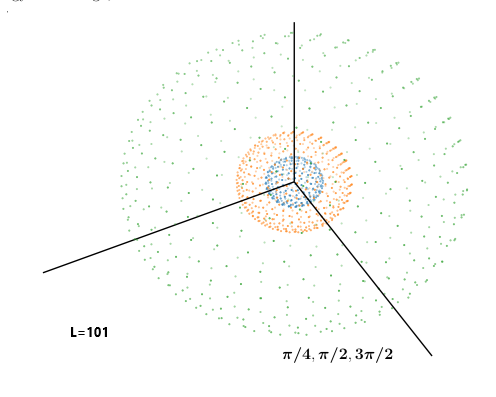
\includegraphics[width=10cm]{fig2}
\caption{The squared sine cloud.}
\footnotesize{Three representative shells with a point distribution proportional to the squared sine are shown here. This sieve is at the core of the harmonic behavior of the toy universe. See Sect.~\ref{subsec:Sine} for further details.}
\label{fig2}
\end{figure}

%%%%%%%% INITIAL STATE %%%%%%%%%%

\section{Initial state}\label{initial-state}

\subsection{Overview}
Among the countless possibilities, we choose the following platonic solution for the initial state problem, described below.

The initial state sets up the configuration of all cells within the lattice. At $t=0$, when all bubbles are superposed at the center ($L/2$, $L/2$, $L$/2), this state is referred to as the \textit{singularity}.

Additionally, the same initialization procedures are mirrored on the draft lattice, ensuring consistency and coherence across both structures.

Although high-level functions and real numbers are used in defining initial states, this does not violate the foundational approach of using natural numbers exclusively in the dynamic process. The real-number values and functions serve only as intermediaries for calculation, while the resulting natural number values are assumed to be imprinted directly onto the space structure by fiat. This approach preserves the integrity of a natural-number-based dynamics, grounding the system’s evolution firmly within the discrete structure of the lattice.

\subsection{Miscellaneous procedures}

First, the vector $\boldsymbol{x}$ is initialized with the appropriate Cartesian positive coordinates ($0 \dots L-1$). These values remain constant but accompany the bubble during relocation. Additionally, the time counters $t$ and $k$ are initialized to zero. The vector $\mathbf{c}$ is also set to zero and the $hBit$ is reset.
 
The weak charge is defined as $w_{0}^{i} = i \,\boldsymbol{\bmod}\, 2$ and $w_{1}^{i} = (i / 2) \land 1$, while the electric charge is given by $q_{i} = w_{1}^{i} \,\boldsymbol{\oplus}\, w_{0}^{i}$ ($i=0...W-1$). The color is determined as $color = i \,\boldsymbol{\bmod}\, 8$. Finally, all bubbles are initialized as $a_{i} = w$. These choices result in a very regular pattern of charge distribution.

This and the following pattern creation are then replicated across all layers in dimension W.

\subsection{Computing the Euclidean distance}
The Euclidean distance is a function of the spatial coordinates given by

\[
d(x,y,z)=int\left(\sqrt{\bigg(x-\frac{L}{2}\bigg)^{2}+\bigg(y-\frac{L}{2}\bigg)^{2}+\bigg(z-\frac{L}{2}\bigg)^{2}}\right).
\]
This justifies, once again, the need to adopt an odd value for $L$: a central point is necessary for this pattern to be properly defined. 

\subsection{Computing the sine cloud} \label{subsec:sine-cloud}
In a 3-torus, the sine squared function will wrap around seamlessly in all three dimensions, ensuring that there are no discontinuities. This property allows for a continuous representation of various physical phenomena across the toroidal structure. Each dimension can be thought of as a periodic loop, where values of the sine squared function are confined within a range that recurs indefinitely. The shell of maximum amplitude must be dense, having all its $\phi B$ bits turned on.

Appendix \ref{sec:pBits-sBits} will compute the pBit and sBit bits—essentially linear and spiral bit patterns with distinct orientations in each layer.

With the full initialization complete—included the setup of spatial coordinates, charge distributions, pBit and sBit vectors, and timing variables—the system is ready to evolve dynamically. The following section introduces the operational heart of the model: the light frame. This framework governs the evolution of bubbles across the lattice through a cyclic sequence of interaction, propagation, and relocation steps. It is within this structured loop that particles begin to move, interact, and display emergent physical behavior.

%%%%%%%% THE LIGHT FRAME %%%%%%%%%%

\section{The light frame}\label{sec:light-frame}

The light frame (shown in Figure \ref{fig:light_frame}) is divided into four steps: Convolution, Diffusion, Relocation, and Transport. Let us first consider some definitions.

\begin{figure}
\centering

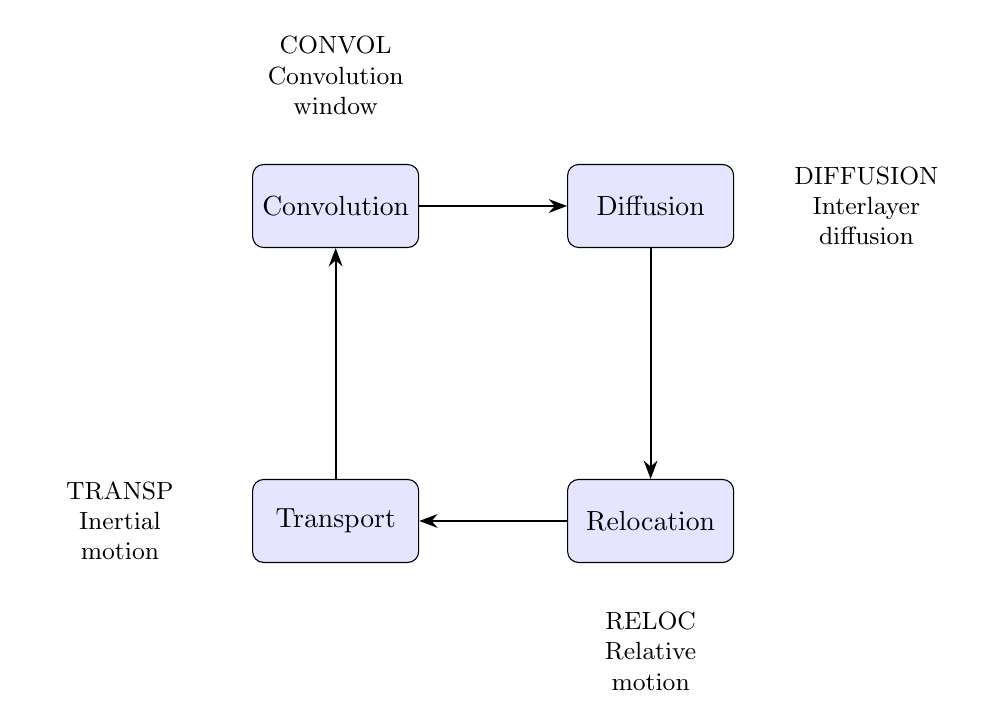
\begin{tikzpicture}[
    process/.style={rectangle, rounded corners, minimum height=3em, minimum width=6em, text centered, draw=black, fill=blue!10},
    arrow/.style={-Stealth, thick},
    annotation/.style={text width=6em, font=\small, align=center}
]

% Define the nodes for each step
\node[process] (convolution) at (0,0) {Convolution};
\node[process] (diffusion) at (4,0) {Diffusion};
\node[process] (relocation) at (4,-4) {Relocation};
\node[process] (transport) at (0,-4) {Transport};

% Draw arrows to indicate the cyclic process
\draw[arrow] (convolution) -- (diffusion) node[midway, above] {};
\draw[arrow] (diffusion) -- (relocation);
\draw[arrow] (relocation) -- (transport);
\draw[arrow] (transport) -- (convolution) node[midway, left] {};

% Add annotations for constants
\node[annotation, above=0.5cm of convolution] (convol-anno) {CONVOL\\ Convolution window};
\node[annotation, right=0.5cm of diffusion] (diff-anno) {DIFFUSION\\ Interlayer diffusion};
\node[annotation, below=0.5cm of relocation] (reloc-anno) {RELOC\\ Relative motion};
\node[annotation, left=0.5cm of transport] (trans-anno) {TRANSP\\ Inertial motion};

\end{tikzpicture}
\caption{The Light Frame cycle of the cellular automaton model, illustrating the sequential steps of Convolution, Diffusion, Relocation, and Transport. Each step is governed by key constants (CONVOL, DIFFUSION, RELOC, TRANSP) that manage bubble interactions and propagation across the lattice, enabling emergent physical behaviors.}
\label{fig:light_frame}
\end{figure}

\subsection{Definitions\label{subsec:Definitions}}

Let us define the following natural constants related to the light frame and interactions:

\begin{itemize}
\item \textbf{DIAG}\\
Defined as $ \lfloor \sqrt{3} \cdot L \rfloor$, this constant measures the diagonal length of the 3D lattice. It is useful for determining maximum interaction distances within the lattice.

\item \textbf{RMAX}\\
Defined as $DIAG/2$, it represents half the diagonal length of the lattice, setting a maximum radius a bubble can achieve before wrapping itself.

\item \textbf{CONVOL}\\
Represents the convolution window, defined as $W$. This constant determines the range in which the initial convolution process is performed during the light cycle.

\item \textbf{DIFFUSION} \\
Defined as \(CONVOL + W - 1\), this constant specifies the maximum diffusion range along the \(W\) dimension during a collapse event. It acts as a preparatory step for relocation if any collapse bit is true at the start, then by the end, all layers are aware of an imminent collapse.

\item \textbf{RELOC}\\
This constant, defined adding $(L-1)$ ticks to the diffusion step, specifies the region dedicated to bubble relocation after initial interactions and diffusion have taken place. It ensures that any necessary adjustments to the positions of particles are made.

\item \textbf{TRANSP} \\  
This constant, defined by adding \(3\cdot (L-1)\) ticks to the relocation step, complement the relocation process in the event of inertial transport.

\item \textbf{FRAME}\\
This constant holds the same value as $TRANSP$, but its semantics differ. It represents the total duration of the light step, encompassing all phases: convolution, diffusion, transport, and relocation.

\end{itemize}

\subsection{Bubble, pair, singleton, and blob} \label{subsec:pairs}

A \emph{bubble} is an expanding spherical wavefront of information organized across cells within a common layer. Spherical propagation is determined by comparing the Euclidean distance $d$, precomputed and stored in each cell, to the evolution parameter $t$. 

\subsubsection{Pair}
Two bubbles are overlapping if they share the same spatial coordinates and $t_1=t_2$. Overlapping bubbles can form a \emph{pair} if they have the same affinity, that is, $a_1=a_2$.

\subsubsection{Propeller} \label{subsubsec:propeller}
A distinct kinematic role of a pair is that of a \textit{propeller}, which continuously repositions other bubbles, forming the fundamental mechanism for inertia and motion, as will be clear later.

\subsubsection{Singleton}
A bubble that does not form a pair is called a \textit{singleton}.

\subsubsection{Blob}
The \textit{blob} is a group of superposed pairs having the same affinity and the same (active) pBits.

\subsubsection{Specialized pairs} \label{subsec:specialized-pairs}
Certain pair combinations are not allowed to form blobs: 

\begin{itemize}
    \item Neutrino and antineutrino pairs possess color values $N, N$ and $\bar{N}, \bar{N}$, respectively.

    \item The up quark fragments $u$ exhibit equal, nontrivial colors and a positive charge in the case of Orbis. 

    \item The propeller adds to the relativistic mass of the propelled fermion, as will be seen ahead.\footnote{This reflects a Kantian view in which particles do not possess self-motion but require an external cause—here, the interaction with fragments—to change their state of motion.}

    \item Pairs that exhibit full complementary charges are termed \emph{gravitons}. These pairs can operate in both Orbis and Umbra.\footnote{Clearly, Orbis and Umbra coexist spatially.}. Each graviton pair has a fixed, absolute, oscillation frequency of $2$. Gravitons contribute to the static interactions in both sectors. Without the graviton, matter from Umbra would appear entirely inert in Orbis, and gravity would not exist. The mechanism by which gravitons contribute to gravitational interactions is further elaborated in Sect. \ref{subsec:emergence-of-gravity}.
\end{itemize}

\subsection{Interaction principles}
Even before considering the light frame itself, let us discuss a few guiding principles adopted.

\subsubsection{Wavefronts clash}
The wavefronts of the interacting bubbles must be active. That is, the expression $d_1 = t_1 \wedge d_2 = t_2$ must hold. In everything that follows, this condition is taken for granted.

\subsubsection{Aggregation and dissolution}\label{subsec-role-of-affinity}

As bubbles interact, they may aggregate by sharing a common affinity, thereby forming particles (see Sect. \ref{sec:Particles} for a deeper definition). The general rule is: the smallest affinity value prevails $a_1=a_2=min(a_1,a_2)$ . When particles dissolve, they assume their layer indices $a_1 = w_1, \, a_2 = w_2$. If the interaction is between a singleton and a pair, then the pair takes the affinity of the singleton $a_2^1=a_2^2=a_1$.

Notice that the $min()$ operator above is idempotent and supports closure, making it a good fit for an ontological model of entanglement.

\subsubsection{Charge conjugation}

Charge conjugation is a principle that governs interactions between bubbles in the CA. Charges impose specific constraints on one another, ensuring that interactions occur in well-defined ways, ultimately aiming for neutrality.

Neutrality can be defined either for an isolated bubble or for a pair of bubbles. For electric charge, represented by a single bit, neutrality can only be established for a pair of bubbles with opposite charges, resulting in net neutrality. Since an isolated bubble contains only one electric bit, neutrality cannot be defined in such a case.

For weak charge, represented by two bits, neutrality arises from how the pair of weak bits combines to determine handedness in both the \textit{Orbis} and \textit{Umbra} sectors.

In the case of the strong force, which utilizes three bits, inner neutrality corresponds to the state \(000\), while inner anti-neutrality corresponds to \(111\). A pair of bubbles with complementary color bits (e.g., \(101\) and \(010\)) also exhibits net neutrality.

The general rule for interactions is then that the resulting combination of charges must achieve a neutral state.

\subsubsection{Pair x singleton interaction}
An interaction of the form $(pB_1\wedge pB_2)\vee (\overline{sB_1}\wedge\overline{sB_2}))\wedge s_1\wedge s_2$ provokes collapse, so $kB_1=1,kB_2=1$. In the other cases, the interaction is triggered by the singleton's pBit.

If only the pBit of one bubble meets the surface of another bubble, we have an adiabatic interaction: there is no collapse. In this case, the affinity and time properties are exchanged, and the bubbles relocate to the other's center. The values of $a$ and $t$ spread to all layer's cells during this relocation.

\subsection{Convolution} \label{subsec:convolution}
Convolution is the first step in the light frame. It ends at the CONVOL tick. It contains the main interaction rules. During this phase, the mirrored image of the main lattice generated in the swapping phase (Sect. \ref{subsec:updating}) is used as follows. Each site in the main lattice is compared to a site in the mirror lattice in dimension $W$, in a circular fashion. The algorithm shown in Appendix \ref{sec:algorithms} shows the main logic adopted. Also during this step, as the pairs are being identified and stacked, the angle $f$ that selects the squared sine point density is incremented accordingly (multiple values of $t$). This angle reflects the notion of frequency.

The formation (or reformation) of particles occurs in the convolution step.

The comparisons are divided into two main groups: the bubbles are superimposing, or the bubbles have distinct origins.

\subsubsection{Superposing bubbles}
Two overlapping bubbles with $f=t$ can form a pair if they satisfy the following conditions:
\begin{itemize}
% Rule 1
\item
$ (q_a \oplus q_b) \land (w1_a \oplus w1_b) \land (w0_a \oplus w0_b) \land (c2_a \oplus c2_b) \land (c1_a \oplus c1_b) \land (c0_a \oplus c0_b) $
\item

% Rule 2
$ (q_a \oplus q_b) \land (w1_a = w1_b) \land (w0_a \oplus w0_b) \land (c2_a \oplus c2_b) \land (c1_a \oplus c1_b) \land (c0_a \oplus c0_b) $
\item

% falta o gluon e os bosons fracos!!!!!!
% Rule 3
$ ch_a = ch_b = 000000\mathrm{B} $
\item

% Rule 4
$ ch_a = ch_b = 111111\mathrm{B} $
\item

% Rule 5
$ (q_a = q_b = 0) \land (w1_a = w1_b = 0) \land (w0_a = w0_b = 1) \land (color_a = color_b) \land (color_a \neq 000\mathrm{B} \land color_a \neq 111\mathrm{B}) $
\item

% Rule 6
$ (q_a = q_b = 1) \land (w1_a = w1_b = 1) \land (w0_a = w0_b = 0) \land (color_a = color_b) \land (color_a \neq 000\mathrm{B} \land color_a \neq 111\mathrm{B}) $

\end{itemize}

These rules implement the formation of pairs, as defined in Sect. \ref{subsec:pairs}. If pairs are detected, we have $f=f+t$. That is, the sine angle is updated. The $hB$ is updated as $hB'=hB$ $\textbf{and}$ $\phi B$

The formation of blobs is made during this step too. Pairs are allowed to superpose if they are equal and were formed by the two first rules above.

\subsubsection{Distinct bubbles} \label{subsec:distinct}
A number of potential interactions may occur when the bubbles are distinct. The algorithm referred to above shows schematically how it happens in most cases.

If two same-sector singletons have opposite charges and both $kB$ bits false, we have annihilation, with both bubbles being reissued from the contact point and their affinity receiving their default values. Both $kB$ bits turn true, triggering a collapse.

If the two singletons share the same affinity, but have different charges, then the singleton whose pBit is the contact point is reissued from the contact point. The other bubble is reissued from the inertial-transported pBit.

If the charges of two singletons are equal and the pBit of the first bubble hits any point of the active surface of the second bubble, then we have fermionic cohesion. The bubbles receive the same affinity; the first bubble is re-emitted from the contact point, while the second from its active sBit cell.

\subsection{Diffusion}

This step propagates information required for the next relocation step, spreading first through the \(W\) dimension and then to all affected layers, ending at the DIFFUSION tick.

If any collapse bit \(kB\) is true at the beginning, then by the end all collapse bits will be true for all bubbles sharing a common affinity. This ensures that all bubbles forming a collapsing particle are identified. In addition, the \(f\) variable propagates according to the rule \(f_{\text{draft}} = \max(f_1,f_2)\). As stated earlier, \(f\) dictates the behavior of photons and other bosons, whose frequencies are multiples of the fundamental cycle. This accelerated time is used to find a suitable point in the sine sieve to allow interaction, defining a concentric bubble. The point found in the sieve (\(f=d\)) must then propagate to the cells in the Euclidean bubble, via the \(hB\) bit, where \(t=d\), so that it can serve as a sieve during this step.

When an interaction is detected, the current value of the \(\mathbf{c}\) vector must be propagated to all cells in the layer in preparation for the massive relocation of data. The rule is: check each neighbor until a nontrivial \(\mathbf{c}\) vector is found and copy its value to the draft cell.

\subsection{Relocation} \label{subsec:relocation}
The final part of the light step addresses bubble relocation itself, building on the diffusion step. It ends at the RELOC tick. Bubbles shift in specific directions (north, west, down) until they have completed their relocation process, including the inertial transport mechanism. The example rule is: if $\textbf{c}_x^{north}>0$, copy the content of the neighbor cell to the draft cell and decrement $\textbf{c}_x$ at the draft cell.

Since wavefront propagation is guided by the Euclidean distance information pre-assigned to each cell, when a bubble is re-emitted due to interaction with other bubbles, all pertinent cell information must be shifted, or relocated, to the new position determined by the variable $\textbf{c}$. This ensures that the bubbles are relatively displaced with respect to each other. The final operation sets $t=0$ at the center cell of the relocated pattern. Relocation is the main consequence of an interaction.

Bubbles are re-emitted either immediately after an interaction or through wrapping. When the bubble is reissued, the previous wavefront continues to propagate until it fades through wrapping. In this state, the bubble is referred to as an \textit{orphan}, meaning it has affinity disabled but is still capable of non-collapsing interactions. In this case, $a=W$ for the outer cells, set during the relocation step. 

To complete, the diffusion of the time variable $t$ occurs here at the last tick: When a cell has a neighboring cell with a lower $t$ value, it updates its own $t$ variable to match the lower value. With this rule, the relocated bubble is capable of expanding again. This timing is crucial to avoid the 'clean diamond' pattern with the new values overrunning the orphaned data.

When the relocation is complete, bubble variables are prepared for the next cycle. If the time frame completes, the $k$ counter resets to zero, preparing the system for the next iteration.  At the conclusion of the process, all $\boldsymbol{c}$ vectors will have a null value.

A bubble can only be relocated to a point on its active surface. This guarantees that the speed of light will never be violated. 

When two bubbles interact, four relocation options are possible:

\begin{enumerate}
\item Both are relocated to the contact point.
    \item One is relocated to the contact point, while the other to its $pB$ bit cell.
    \item One is relocated to the contact point, while the other to its $sB$ bit cell.
    \item Obeying the inertial transport rules described in Sect. \ref{subsec:inertial-transport}.
\end{enumerate}

\subsection{Main lattice updating and mirroring} \label{subsec:updating}
After each tick of the $k$ clock, with a total duration of FRAME ticks, the modified data in draft must be transferred at once to the main lattice. First, if the $k$ counter is within the $CONVOL$ window, the draft lattices are shifted in the $W$ dimension to disalign them from the current draft lattices to convolute.

The current lattices then receive the content of their draft lattices. Also, at the beginning of the evolution step, the mirror lattices are also massively updated with the current lattices' content, thereby preparing the system for comparisons in the $W$ dimension at the next convolution phase (Sect. \ref{subsec:convolution}). The $f$ variable of the mirror lattice receives the same value as $t$, that is, $f_i^{mirror}=t_i^{main}$.

%%%%%%%% INTERACTIONS %%%%%%%%%%

\section{Interaction details\label{sec:Interactions}}

Some aspects of the interactions detected during the convolution step will now be elucidated.

\subsection{The role of the sinusoidal sieve}

The $\phi Bits$ cloud, together with the $kB$ bit dictate the harmonic behavior of the model. This sieve mechanism is used in electrical and weak interactions only and is assumed to be used henceforth. It helps to explain why the strong force is stronger than the electroweak force.

\subsection{Inertial transport} \label{subsec:inertial-transport}

Inertia is acquired by an inertial transport mechanism. It completes at the TRANSP tick. It happens between two bubbles with the same affinity when the pBit of one bubble hits the surface of the other bubble. One bubble is reissued from $\boldsymbol{x1}$, while the other from $(\boldsymbol{x_1}-\boldsymbol{x_2})\,\boldsymbol{mod}\,L$.

The propeller (see Sect. \ref{subsubsec:propeller}) naturally emerges as a pair in order to avoid static interaction. It represents a fragment of a photon or of a graviton, where the pair exhibits symmetric charges. This symmetry effectively bypasses the priority of interactions mediated by forces such as the Coulomb force. 

Furthermore, when a photon blob interacts in this manner—acting as a propeller, a specific pair detaches from the photon to become a distinct propeller.

\subsection{Charge combination}

The $w_{1}$ weak charge bit separates the interactions into two groups:
same-sector and inter-sector. We will first describe the same-sector ($w_{1}^{1}=w_{1}^{2}$) cases and later the inter-sector case in what follows.

\subsubsection{Static interactions}

Let two electric charges, $q_1$ and $q_2$, from two distinct particles, be placed at a distance from each other. A static interaction, namely the Coulomb or magnetic force, begins with the direct alignment of an orphan singleton from $q_1$ with a graviton from the vacuum, both being reissued at the contact point. If this graviton interacts with $q_2$, it is then reissued at that point, acquiring the affinity of $q_2$. That is, gravitons are reissued along the path of a flux of orphan singletons from particle $1$, increasing the probability of interacting with $q_2$ in that region, and becoming one of its propellers. The same is valid the other way around.

\subsubsection{Coulomb interaction} \label{subsec:Coulomb-interaction}

Coulomb attraction and repulsion occur in two steps: a) the pBit of an orphan of the first charged particle hits an active cell of a graviton. If they are aligned or antialigned (checking their $x$ vectors), the graviton is reissued from the contact point, carrying the affinity of the orphan, in this case W; b) then, the $pB$ bit of the second charged particle, which was aligned with the graviton, hits an active cell of the graviton being reissued, carrying the affinity of the singleton, that is, it becomes a propeller with the correct direction.

\subsubsection{Static magnetic interaction}

The magnetic case involves the $sB$ instead of the $pB$. It is valid for interactions between electrons, quarks, and W bosons.

The emphasis of propellers on the pBit rather than the sBit significantly influences the resulting propeller: the faster the particle moves, the more likely it is to be perpendicular to its direction of motion.

\subsubsection{Neutrino interactions}

Let $q_{0,1}$ be a pair of complementary electrical bits. A neutrino fragment is a pair of bubbles with charge content $q_{0,1} = 00000B$, while an antineutrino fragment is a pair with both bubbles having charge $q_{0,1} = 01111B$. (Anti)neutrino fragments interact with (right)left-handed particles only.

\subsubsection{The up quark and down quark fragments}

We can behold possible combinations of color properties between pairs of bubbles in the table of Fig. \ref{fig:color-combination}. (Anti)\emph{quark} fragments have non-trivial color and are marked as $q$ or $\bar{q}$, (anti)neutrinos are $\nu$ and $\bar{\nu}$, gluons are $g$, and photons are $\gamma$. Since half the gluon fragments are right-handed, they are shown as photons. The cells marked as blue, if having both quarks with electrical charge $q=+$, may form an \emph{up quark}
fragment. 

An \emph{up quark} (\emph{u}) can be any of the \emph{+R+R}, \emph{+G+G} or \emph{+B+B} fragment pairs, while a \emph{down quark} (\emph{d}) can be any of the \emph{-R, -G or -B }single fragments. When we combine three of these quark fragments into a \emph{proton} fragment \emph{uud}, we get an uncompensated color. The matter end of the gluon may fit this lack, but in return it generates an antimatter end, and so on, in a dynamic balance. In consequence, it follows that the \emph{electron} fragment must be -N,-N,-N.\footnote{This explains the fractional charge of quarks.} 

An important remark fits here: the quantity of up quark fragments in each sector is crucial in defining an upper limit for the production of protons and, consequently, \textit{atoms}.

\subsubsection{Symmetry breaking after singularity}

At the singularity (initial state), all bubbles overlap, necessitating an additional interaction rule to achieve separation. The adopted rule is as follows:

During the convolution step, if a spatial address contains two overlapping bubbles with fully symmetric charges, the bubbles are reissued from their respective active pBit sites. This process rapidly disperses the singularity, facilitating the separation of Orbis from Umbra. Let us call this \textit{segregation}.

By the simple fact that $W$ is an odd number, if we try to form pairs from different layers, an ultimate singleton will automatically remain. Let's call it the \textit{rebel}.

In the next light step, there will be two large groups of pairs and a single singleton—the rebel—definitively breaking the original symmetry and triggering an initially chaotic evolution.

\subsubsection{Singularization}
The counterpart to segregation is singularization. In the distinct case (Sect. \ref{subsec:distinct}), partners with fully complementary charges are reissued from a single active pBit site.

\subsection{Annihilation and collapse}

The destruction of a particle due to annihilation or collapsing light-matter interaction is also performed during the convolution step, but only in the annihilation case, the affinity properties will be redefined to their default values $a_w=w$, where $w$ represents the index of the $W$ dimension. Bubbles are now raw materials for the formation (or recreation) of new particles in this case.

One direct consequence of this ontological collapse mechanism is the presence of an arrow of time at the fundamental level, and thereby it reinforces the second law of thermodynamics. This also pushes the occurrence of a Poincaré cycle to the distant future (see Sect. \ref{sec-undecidability}).

\subsection{Self-interference\label{subsec:Interference}}

As previously discussed, space in this model possesses a memory that records the trajectories of particles, giving rise to the phenomenon of self-interference—reminiscent of the double-slit experiment with fermions \cite{feynman-2}. This idea is inspired by the approach proposed by Sciarretta in \cite{sciarretta}, which uses punctiform stochastic particles to account for interference.

The central mechanism involves leaving a trace of a particle’s history in the lattice as its bubbles propagate through space under the action of propellers. This trace is encoded by the last affinity value $a$ and the most recent sine phase $f$ left behind in the visited cells.

During the convolution step (see Sect. \ref{subsec:convolution}), the system compares the properties of incoming and residual bubbles. If the equality $d = t$ holds, indicating synchronized timing, standard cohesion occurs. In contrast, if $d=f$ holds, only the new bubble is reissued, altering the fermion’s dynamics and generating interference patterns as a consequence.

This memory-based mechanism enables temporally shifted interactions among the constituent fragments—effectively the 'bits'—of qubits (see Sect.~\ref{subsection:qubits}), thereby providing a natural substrate for complex quantum behavior to emerge from a fundamentally discrete framework.

We are now ready to infer how particles emerge from these low-level rules.

\begin{figure}
\caption{Color combination.\label{fig:color-combination}}
\medskip{}

\begin{centering}
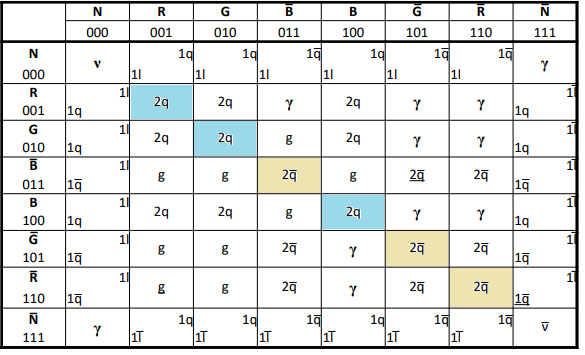
\includegraphics[width=\linewidth]{fig4}
\par\end{centering}
\medskip{}

{\small{}Possible combinations of colored fragments are shown, where (anti)quark fragments are marked $q$ and $\bar{q}$, (anti)neutrinos are $\nu$ and $\bar{\nu}$, gluons are $g$, and photons are $\gamma$. Since half the gluon fragments are right handed, they are shown as photons. The cells marked as blue, if having electric charge $q=+$, may form an }\emph{\small{}up quark}{\small{} fragment in Orbis.}{\small\par}
\end{figure}

%%%%%%%% PARTICLES %%%%%%%%%%

\section{Particles\label{sec:Particles}}

Bubbles form the composite structure of particles, which can be studied through experimental physics. A particle is characterized not only by the proximity of its bubbles but primarily by the fact that most of these bubbles share the same affinity value \( a \). Electrical charge quantization has a fundamental role in the formation of localized particles; that is, the number of similar singletons in a particle is $N_e$ on average, besides its swarm of propellers.

The action of the weak or strong charge (but not the electric charge) is inhibited in a pair if their components are complementary. Both bubbles are reissued in an interaction involving a pair. In general, the combinations formed correspond to boson fragments.

\subsection{Fermions}
A particle is classified as a fermion when its structure contains more than just paired kinematic components. Fermions typically exhibit a balanced average of bubbles with identical charges (the up quark is a specialized pair treated in Sect. \ref{subsec:specialized-pairs}), sustained through dynamic charge quantization (see Sect. \ref{subsec:charge-quantization}). Additionally, fermions certainly include pairs that act as propellers, responsible for its inertial movement. Overall, fermions form a small, undetectable volume, "punctiform" cloud of bubbles, surrounded by concentric orphans created through frequent reissues, thus establishing their \textit{field}.
 
Quark confinement originates from the prioritization given to color cohesion and quark-gluon interaction over other forces. In contrast, within an atom, electrons naturally distribute around the nucleus according to spherical harmonic distributions.

Note that specialized pairs, unlike bosons, do not form blobs, giving them a fermionic character. The neutrino pair is an example. Inter-sector neutrino pairs are unique in that they do not interact via the weak force, rendering them sterile in this sense. The small mass of neutrinos is the sum of their two components and additional contributions from propellers (relativistic mass).

\subsection{Bosons}\label{bosons}
A particle is classified as a boson if it is made of one or more blobs. Specific types of pairs that fulfill this criterion include a photon fragment and other gauge-boson fragments. Each of these roles involves a pair structure where some or all charge bits differ except for the $w_{1}$ bit; that is, they are sectorial particles. 

The defining characteristic of a photon is that all its pairs are superposed at the same point, forming a single blob. In contrast, for other bosons, such as the $W^{\pm}$ and $Z$ bosons, in which the pairs form a "punctiform" cloud of multiple blobs sharing the same affinity, somewhat similar to the behavior observed in fermions. At last, the model suggests that the Higgs boson is formed by two $Z^0$ bosons with opposite spins, with no apparent relation to giving mass to other particles.

An orphan (see Sect. \ref{subsec:relocation}) does not interact with photons, because $a=W$, but interacts with gravitons. Neutral orphan pairs do not interact electromagnetically.

%%%%%%%% RESULTS %%%%%%%%%%

\section{Results}\label{sec:Results}

To illustrate the concepts discussed thus far, we have developed a few practical examples.

\subsection{The speed of light and the size of the universe}

We can now state the following constraint on the fundamental quantities:

\[
\frac{X}{\mathcal{L}}=c,
\]
where $c$ is the speed of light and $\mathcal{L}$ is the number of ticks per frame. Estimates for the values of \emph{X} and \emph{L }(truncated to a natural) are taken from Appendix \ref{sec:Calculation-of-X}

\[
X=l_{P}
\]
and

\[
L\approx6.95410\times10^{60}\approx2^{202},
\]
where $l_{P}$ is the Planck length. From this, we calculated the size of the universe as $1.94669\times10^{26}\,m$ (the \emph{Grand Cube} diagonal).

\subsection{A charge conjugation study}

A small program (see Ref. \cite{af_neto}, file \emph{combine.c}) was created to check the combination of charges. A total of $6\times32768=196,608$ fragments, with their charges evenly distributed, were randomly combined in several million attempts, and the averages tabulated. It was assumed that only 'hydrogen atoms' are formed.

Since the strong force dominates, a probability value of 0.001 was assigned to the search for up quarks and 0.999 to gluons. These values were calculated based on the smallest possible set of charges. The search was conducted in four stages. First, gluons and up quark fragments were targeted (fragments of electrons were also included, as their existence depends on the number of generated up quarks). Next, photons and neutrinos were sought, followed by fragments of the W and Z bosons, and finally, anti-atoms were examined.

The results can be seen in Table \ref{combina}. The leftover, that is, the bubbles that could not form a pair or a singleton, reveal a highly ionized environment, which will be attenuated by inter-sector interactions, resulting in an increase in the photon count. These data resemble roughly a few simple 'atoms', while the photon fragments could form a few multiple pair photons. One can then speculate that the unmatched quark fragments could form mesons or virtual quarks or even contribute to dark matter (50\% + 25\%), and that the Umbra contains more antimatter than Orbis. All in all, it makes sense as a toy universe. 

Interestingly, the proton-electron mass ratio appears in this naive analysis with a value of $1187$ for both sectors, somewhat close to the empirical value of $\approx1836$ (CODATA \cite{codata}). 

\begin{table}
\caption{Charge combination}

\medskip{}
\label{combina}
\begin{centering}
{\small{}}%
\begin{tabular}{|l|c|r|r|l|}
\hline 
\textbf{\small{}Fragment} & \textbf{\small{}Type} & \textbf{\small{}Orbis} & \textbf{Umbra} & \textbf{\small{}Obs.}\tabularnewline
\hline 
\hline 
{\small{}Gluon} & {\small{}Pair} & {\small{}3,6760.0} & {\small{}3,6760.0} & \tabularnewline
\hline 
{\small{}Up quark} & {\small{}Pair} & {\small{}42.0} & {\small{}42.0} & \tabularnewline
\hline 
{\small{}Down quark} & {\small{}Single} & {\small{}10.0} & {\small{}10.0} & \tabularnewline
\hline 
{\small{}Electron} & {\small{}Single} & {\small{}31.0} & {\small{}31.0} & \tabularnewline
\hline 
{\small{}Photon} & {\small{}Pair} & {\small{}20.0} & {\small{}20.0} & \tabularnewline
\hline 
{\small{}Graviton} & {\small{}Pair} & {\small{}12.0} & {\small{}12.0} & \tabularnewline
\hline 
{\small{}Z boson} & {\small{}Pair} & {\small{}24,592.0} & {\small{}18,416.0} & \tabularnewline
\hline 
{\small{}W boson} & {\small{}Pair} & {\small{}6,122.0} & {\small{}12,294.0} & \tabularnewline
\hline 
{\small{}Neutrino} & {\small{}Pair} & {\small{}6,082.0} & {\small{}6,082.0} & \tabularnewline
\hline 
{\small{}Antiup} & {\small{}Pair} & {\small{}2.0} & {\small{}2.0} & \tabularnewline
\hline 
{\small{}Antielectron} & {\small{}Single} & {\small{}1.0} & {\small{}0.0} & \tabularnewline
\hline 
{\small{}Antiquark} & {\small{}Single} & {\small{}0.0} & {\small{}0.0} & \tabularnewline
\hline 
{\small{}Leftover} & {\small{}Single} & {\small{}24,624.0} & {\small{}24,620.0} & {\small{}Adds to dark matter}\tabularnewline
\hline 
\textbf{\small{}Total} &  & \multicolumn{2}{r|}{\textbf{\small{}196,602.0 }} & \tabularnewline
\hline 
\end{tabular}{\small\par}
\par\end{centering}
\medskip{}

{\small{}A total of 196,608 bubbles were randomly combined into several million attempts in a small program focused on charges alone (See Sect. \ref{sec:Results} for more details).}{\small\par}
\end{table}

The following section discusses potential challenges and limitations of this approach.

%%%%%%%% CELLULAR AUTOMATA AND QUANTUM FORMALISM %%%%%%%%%%

\section{Cellular automata and quantum formalism} \label{sec:bridge}How can this model be used anyway? For local events, our guide to an answer comes from 't Hooft's seminal work about cellular automata as world models \cite{thooft}.

Of course, the ontological states ($\mathcal{OS}$) representing each configuration of the CA cells cannot form superpositions, since ontological states evolve into ontological states. But, an orthonormal set of ontological states can be used as a basis for a Hilbert space, each represented by a unit vector.

Given a subsystem of the universal automaton, the general recipe for analyzing it using operator mechanics is as follows:

\begin{itemize}
    \item Find a permutation operator as a matrix containing a single 1 in any row or column.
    \item Diagonalize it, obtaining the eigenvalues and eigenvector matrices.
    \item Identify a Hamiltonian matrix as the exponent in $\hat{U}=e^{-i\hat{H}T}$.
    \item Use the eigenvalue matrix to bring this Hamiltonian back to the ontological basis.
    \item Form linear combinations of the ontological states $\ket{A}$.
\[
\ket{\psi} = \sum_A \lambda_A \ket{A}, \quad \sum_A |\lambda_A|^2 \equiv 1,
\]
where $\ket{\psi}$ is a quantum state or "template," and $\lambda_A$ is a complex coefficient.
\end{itemize}

Now, we can use the operator mechanics machinery, in particular the Schrödinger equation, to analyze it:

\[
\frac{d}{dt}\ket{\psi} = -i\hat{H}\ket{\psi}.
\]
Then, the wave function evolves deterministically.

Furthermore, the Born rule can be deduced once we accept the existence of superposition states. It extends ordinary classical probability theory through suitable mathematical treatment. Then, it can be used to predict the final eigenstate (i.e., the collapse) resulting from a measurement.

This is, naturally, a simplified picture. More details can be found in References \cite{thooft,Elze2019,rizzo2020perturbing}.

%%%%%%%% PROSPECTS AND CONJECTURES %%%%%%%%%%

\section{Conjectures and prospects\label{sec:Prospects-and-conjectures}}

This work represents the tip of the iceberg. The challenge now is to delve into the many conjectures that emerge from it, prove them, perhaps with minor adjustments.

Just a few examples are considered here.

\subsection{Charge quantization} \label{subsec:charge-quantization}

A subtle geometric "defect" emerges during the initialization of the CA model (see Sect.~\ref{initial-state}). When attempting to define the pBit lines and sBit spirals as isotropically distributed within the lattice's discrete, square-like constraints, unavoidable asymmetries arise. Specifically, the mismatch between the chosen $W$ dimension ($3\cdot L^2$) and the number of isotropic directions ($\pi\cdot L^2$) introduces a structural defect. Rather than being problematic, this defect acts as a useful artifact—enabling the emergence of quantization, in a manner reminiscent of electric charge quantization in physical systems.

A key mathematical foundation for this quantization lies in the concept of the winding number—a topological invariant that counts how many times a vector field wraps around a point or axis. In the CA model, the defect-induced asymmetries naturally associate with a nonzero winding number, effectively enforcing the discreteness of the system’s state space.

This quantization discretizes the system's possible states, suppressing chaotic evolution and promoting periodic behavior. On smaller grids, it manifests as localized, stable patterns. As the grid scales up, these quantized states remain robust, supporting scalable periodicity and recurring cycles even in larger systems. At this stage, these 'islands' of stability become rigidly organized in a highly regular distribution. How can this positional trend be made more flexible?

To achieve an effective charge quantization—and by extension, the quantization of other fundamental properties—the model requires a mechanism analogous to Dirac's magnetic monopole. In our discrete 3-torus framework, this is realized by ensuring that the property vector $sB$ exhibits non-trivial winding around at least one of the torus’s non-contractible loops. This behavior mirrors the effect of a magnetic monopole in conventional theories, which enforces the quantization of electric charge \cite{dirac1931}. As a result, the "islands", made of $N_e$ bubbles on average, become even more spatially independent and well-defined.

It is important to note that this quantization is only possible due to the separation between Orbis and Umbra, distinguished by the $w1$ bit (see Sect. \ref{subsec:all-dirs}), resulting in a complementary couple of magnetic monopoles. The complementary asymmetries manifest independently within each sector.

Proving this conjecture—and, for instance, calculating the Planck constant from the number of "bubbles" $N_e$ constituting an electron—remains one of the main challenges for future research.

\subsection{Discrete to continuous transition}

The emergence of localized particles as assemblies of numerous discrete fragments implies that their macroscopic properties—such as total momentum and angular momentum—are not defined at the level of individual fragments but arise from collective configurations. Consequently, these global properties are best represented not by discrete values but by real numbers. This shift reflects a transition from fundamentally discrete dynamics to effectively continuous observables. In particular, the summation over a large number of discrete events naturally approximates continuous quantities, mirroring how statistical mechanics bridges atomic behavior and thermodynamic laws. Hence, the discrete underpinnings of the model give rise to continuous behavior at larger scales, aligning with the continuum formalism of classical and quantum physics.

To illustrate this point, consider a free electron whose average motion follows a direction vector that cannot be expressed solely in terms of discrete modulo-L components. Such behavior highlights the necessity of continuous descriptors when characterizing aggregate properties in a fundamentally discrete framework. Continuous functions and their derivatives are, then, useful idealizations.

\subsection{Color quantization}
Color quantization is an extension of the electromagnetic case. Hadrons form by the simultaneous action of charge quantization and strong cohesion.

\subsection{Weak quantization}
Due to the relatively rare occurrence of weak interactions, the weak quantization manifests itself at a cosmological scale: the relation between the average distance between galaxies and their bulges is constant. Deriving a cosmological constant $\Lambda$ and the respective metric tensor $g_{\mu\nu}$ from this is an intriguing possibility. 

This large-scale granularity could then also be interpreted as gravitational quantization.

\subsection{Emergence of gravity}\label{subsec:emergence-of-gravity}

 The smooth spacetime of general relativity is viewed as an effective, coarse-grained approximation of the fundamental discrete structure considered. The model posits that gravity arises as a residual effect of electromagnetic interactions, emerging naturally within the cellular automaton framework through the interplay of photons and gravitons. Acting as super photons, gravitons possess properties that allow them to mediate interactions across the two overlapping sectors of the toy universe, \emph{Orbis} and \emph{Umbra}. While ordinary photons are restricted to sector-specific interactions, gravitons provide a mechanism for fundamental connectivity in a universe otherwise marked by a strong separation between these domains. However, their direct influence on distant masses diminishes due to the cancellation of antagonistic forces (e.g. electric attraction/repulsion) induced by their interactions. What remains is a residual, geometry-driven attractive force \footnote{Recent results confirm that gravity acts attractively on antimatter \cite{anderson2023observation}.} that underpins the emergent gravitational effect. Free objects follow emergent timelike geodesics in this scenario. Through this dual-sector capability, gravitons redistribute energy and charge, also contributing to phenomena analogous to dark matter (flat rotation curves of galaxies).

An additional factor in this framework is the gradual energy dissipation observed as photons travel great distances. This \textit{aging} process, intrinsic to the cellular automaton, parallels photon redshift in its effect. As it propagates, an energetic photon undergoes minor interactions with errant singletons and electrons, without collapsing. Over time, this energy dissipation subtly shifts the light spectrum toward the red end.

The idea was first presented by Zwicky in \cite{zwicky1929redshift}, where he was concerned with the blurring of the received images—a phenomenon that does not occur in our model. Could this effect offer an alternative explanation for cosmic redshift, potentially challenging the need for dark energy?

Note that the propeller turns accelerations equivalent, in particular in the case of the proverbial cabin picturing the GR equivalence principle.

\subsection{Stochastic behavior and the uncertainty principle}

The richness of the regular patterns that intersect to determine an interaction, combined with the large number of bubbles that form the particles, results in seemingly random outcomes, despite the deeply deterministic nature of the model.

This apparent randomness emerges from the richness of the interactions. For example, a coin-flipping-like operation occurs when determining a common affinity (see Sect. \ref{subsec-role-of-affinity}). Since both particles and measurement instruments are composed of many bubbles, each measurement effectively samples a single instance from this distribution. Consequently, there will always be a degree of uncertainty in measured values. In quantum mechanics, this uncertainty is fundamental and manifests as the well-known Heisenberg principle \cite{Heisenberg1927}:

\[
\sigma_x \sigma_p \leq \frac{\hbar}{2}.
\]
Here, the standard deviations $\sigma_x$ and $\sigma_p$ represent the spread of position and momentum measurements.

\subsection{Black holes}
The quintessential idea of a black hole in this model can be illustrated by two electrons, each with radius $R$, so close to each other $d<2R$ that the quantization is broken and they simply fuse, forming a particle with radius $R'=2^{1/3}R$ with a dominant affinity value. 
\[
a_1 = a_2 = min(A_1,A_2).
\]

A picture of the internals of a black hole can then be readily extrapolated from this simple example: a mixture of bubbles, most lacking quantization while others exhibit it incompletely, in a frenetic and densely packed configuration.

It is clear that, in this picture, there is no black hole information paradox \cite{hawking1976breakdown,harlow2016jerusalem}.

\subsection{What is spin in this model?}
In this model, the spin of a localized particle emerges from the preferential alignment of the pBit \( pB \) and its corresponding sBit spiral \( sB \). These bits tend to align either radially outward or inward relative to the particle’s center. This binary emergent behavior defines the two spin states: spin up and spin down, respectively. The alignment occurs consistently across the constituent bubbles of the particle, reflecting a coherent internal structure. The radial axis is defined by the potential $pB$ bits of the layer.

\subsection{The Hofer effect}

A particular challenge, then, is to verify what we call the \emph{Hofer effect}: the expected tendency for all individual 'spins', represented by the direction of the spiral of $sB$ bits, of a localized particle to align radially, either inward or outward (spin up/down), as described above and predicted in Hofer \cite{hofer}. In that work, the author explains how magnetic effects emerge from the symmetry breaking of this spherical pattern, thereby supporting the Stern–Gerlach experiment.

\subsection{Particle zoo panorama}
As it stands, this model serves as a framework to speculate on the composition of known particles. In the discussion that follows, the fragments will be characterized by their charge content: \(q, w1, w0, c2, c1, c0\). For example, we designate the fragment \(100000\) as \(-L\) and \(001111\) as \(-\bar{L}\), and so forth. The following descriptions are expected to occur naturally due to the evolution of the system.

\subsubsection{The electron neutrino}
The electron neutrino $\nu_e$ is formed by a single [$+L:-L$] pair and additional propellers. Yet the anti-electron neutrino $\bar{\nu}$ uses the pair [$+\bar{L}:-\bar{L}$].

\subsubsection{The electron}
The electron $e^-$ is formed by a quantized number of $-L$ fragments, a great number of electron neutrinos $\nu_e$, and a variable number of propellers (see Figure \ref{fig:electron}). The positron, or anti-electron, uses $+\bar{L}$ fragments instead. These are for Orbis, in the case of Umbra, all bits are inverted.

\begin{figure}
\centering
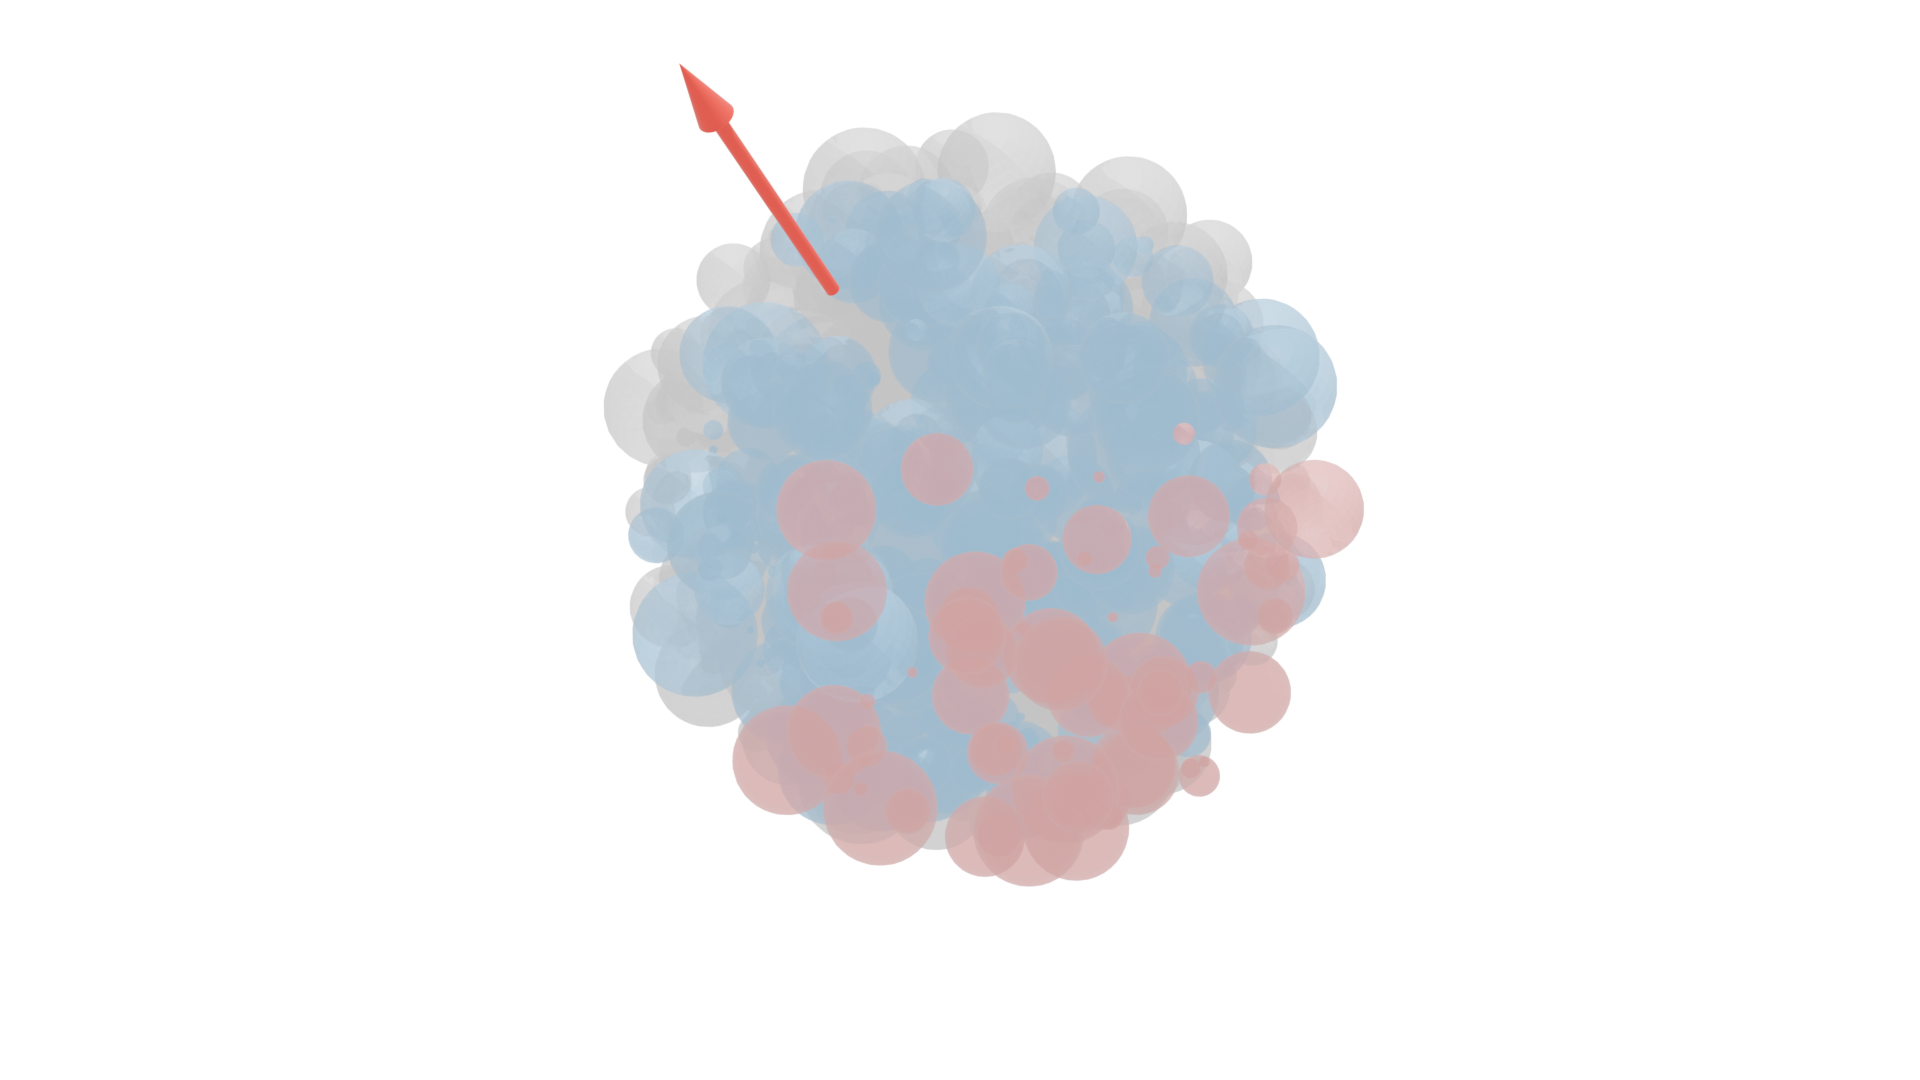
\includegraphics[width=\linewidth]{fig1}
\caption{The free electron.}
\footnotesize{Artistic impression of a free electron. The red bubbles are propellers with a resultant in the direction of the arrow. The blue bubbles are negative charge singletons, while the gray bubbles are electron-neutrino pairs.}
\label{fig:electron}
\end{figure}

\subsubsection{The muon neutrino}
The muon neutrino $\nu_{\mu}$ is formed as $\nu_{\mu}=2\nu_e+\bar{\nu}_e$ plus additional propellers. It is like an electron neutrino, but with a compensated antimatter part.

\subsubsection{The muon}  
The muon $\mu^-$ consists of a quantized number of $-L$ fragments, a large number of muon neutrinos $\nu_{\mu}$, and a variable number of propellers. The classical study conducted by Itô in \cite{ito} suggests that this configuration stabilizes at the second harmonic of the electron's radial vibrational state.

\subsubsection{The tau neutrino}
The tau neutrino $\nu_{\tau}$ is formed as $\nu_{\tau}=3\nu_e+2\bar{\nu}_e$ plus additional propellers. It is also like an electron neutrino, but with a compensated antimatter-enriched part.

\subsubsection{The tau}
The tau $\tau^-$ is formed by a quantized number of $-L$ fragments, a great number of tau neutrinos $\nu_{\mu}$, and a variable number of propellers.

\subsubsection{Gauge bosons}
These bosons were described in Sect. \ref{bosons}.

\subsection{Leptons decay}
In the Standard Model (SM), the decay products typically include one neutrino or antineutrino. However, in our model, the large number of neutrinos is entangled, sharing a common affinity. When one neutrino interacts via the weak force, all other entangled neutrinos collapse to the same point. This phenomenon gives the appearance of a single, energetic neutrino, as the observable outcome remains indistinguishable, in agreement with the SM predictions.

\subsection{Electronic decay}
After the absorption of (part of) a photon, the electron enters an excited state, dynamically stabilizing in a suitable spherical harmonic configuration. When the common components of the photon and electron are reissued, the odds of a configuration corresponding to the original photon are less than one. As time passes, after many cohesion interactions, the proper configuration of charges and pBits may occur, forming a single photonic blob and allowing the emitted photon to escape the frequent reissue mechanism, fleeing away from the electron cloud, which eventually settles into its ground state.

\subsection{Compound particles half-lives}
Protons, electrons, and electron neutrinos are composed exclusively of bubbles, without their corresponding anti-bubbles. This unique composition is a key factor in their exceptionally long half-lives, potentially making them stable. In contrast, particles containing both bubbles and anti-bubbles are significantly less stable. Their shorter half-lives result from the likelihood of annihilation events between bubbles and anti-bubbles within their structure, leading to their transient nature.

The neutron embeds lots of electron antineutrinos, which bind the negative charge to its inner proton. This explains the decay of the free neutron.
\[
n^0\rightarrow\,p^{+}+e^{-}+\nu_e
\]

\subsection{Nuclear decay}

In this model, nuclear decay processes emerge from the internal structure and composition of compound particles representing atomic nuclei. These instabilities trigger reorganizations via the electroweak collapse mechanism, where the sieve test result ($hB$) determines the feasibility of transformations. The decay process is similar to the free neutron decay seen above. The perturbing particles are typically neutrinos and Z bosons that permeate the vacuum.

This internal annihilation mechanism provides a foundational explanation for the decay processes observed in nature, aligning the model with empirical observations of nuclear instability as presented in the well-known tables of nuclides.

\subsection{Heavier quarks}
The framework suggests that the other quarks follow the composition of leptons, with additional neutrinos and antineutrinos, besides a variable number of propellers.

\subsection{Atoms}
Bound states of protons, neutrons, and electrons are naturally expected in this scenario.

\subsection{The abundance of neutrinos}

Despite the relatively small number of neutrinos observed in Table \ref{fig:color-combination}, their large cosmic abundance can be understood in light of their extremely low mass, approximately five million times smaller than the mass of an electron. This characteristic allows neutrinos to exist in enormous quantities across the universe, even if their presence appears limited.

\subsection{Quest for qubits} \label{subsection:qubits}

An electron may be conceived as a vast ensemble of dynamic \textit{nanostates}, collectively manifesting as a single particle through their shared affinity. When two electrons share the same affinity (totally or partially), they become distinguishable only through the constraints imposed by quantization dynamics. However, if one momentarily relaxes these constraints, such a pair can be interpreted as a system of qubits—capable of exhibiting a far richer spectrum of interactions.

What, then, supports this emerging computation? Spatial interaction is facilitated by the convolution step, while the self-interference mechanism (see Sect.~\ref{subsec:Interference}) introduces a form of temporal smearing that allows information to persist and influence future states.

Moreover, the atoms that host these electron structures local space via the SU(3) symmetry induced by the strong charge, further enriching the landscape of possible interactions.

This broader perspective suggests a behavior akin to an intricate network of Turing machines, each representing a potential computational pathway. The computation results are being revealed by interpreting correlations. Such an interpretation may offer new insight into the astonishing experimental results of quantum computing.

\subsection{Observers and spacetime}  

This framework extends Wheeler's "it from bit" concept by providing a mechanism through which information constitutes physical entities, albeit from an omniscient perspective. To address the internal viewpoint, we now define inner observers or simply \textit{observers}. 

\subsubsection{Minimal observer definition}

Here, we formalize the concept of a \emph{minimal observer}, following the framework introduced in Hatem Elshatlawy et al. \cite{elshatlawy2025towards}. A minimal observer is defined as the simplest system capable of performing observation in a functional sense, embodying core components of sensing, internal processing, and acting upon an environment within a closed feedback loop.

\begin{definition}[Minimal Observer]
Let $O$ be a system described by the tuple
\[
O = (X, Y, Z, f, g, B),
\]
where:
\begin{itemize}
    \item $X$: Internal state space (e.g., memory or configuration states),
    \item $Y$: Input (sensor) space,
    \item $Z$: Output (action) space,
    \item $f: X \times Y \rightarrow X$: State transition function (state update rule),
    \item $g: X \rightarrow Z$: Output function (generates actions based on internal state),
    \item $B$: Boundary condition demarcating the internal observer from its external environment.
\end{itemize}

The system $O$ qualifies as a \emph{minimal observer} if it satisfies:
\begin{itemize}
    \item $|Y| \geq 1$: Non-trivial sensing,
    \item $|Z| \geq 1$: Non-trivial actuation,
    \item $|X| > 1$: Non-trivial internal dynamics,
    \item \textbf{Feedback closure:} The output $g(x)$ must influence the environment in such a way that it alters future inputs $y \in Y$.
\end{itemize}
\end{definition}

This definition ensures that the observer possesses the minimal necessary structure to distinguish itself from its environment and engage in interaction through perception and response. Importantly, this framework abstracts away from higher-order capabilities such as memory, learning, or consciousness, focusing instead on the foundational structure that enables observation.

\subsubsection{Spacetime}
As established, the spacetime of this model is inherently flat and regular. However, the spacetime perceived by observers and laboratory instruments appears curved, in accordance with the principles of General Relativity. How can this apparent discrepancy be reconciled?  

The resolution lies in understanding the role of propellers, which contribute both to motion and to mass-energy content. Their interactions create a framework in which observers, laboratory instruments, and the environment mutually influence one another. This interplay generates effective gravitational potentials, causing clocks to tick slower near concentrations of mass. Such behavior unveils a \textit{timescape} scenario \cite{duley2013timescape}, where the perception of curved spacetime naturally emerges from relational dynamics within an underlying flat background.

Given the mutual dependence of all system components and the absence of free external variables, the model aligns with superdeterministic interpretations of reality, as discussed by Hossenfelder and Palmer \cite{hossenfelder2020rethinking}.

%%%%%%%% CONCLUSION %%%%%%%%%%

\section{Conclusion\label{sec:Discussion}}

\subsection{Undecidability and long-term dynamics}\label{sec-undecidability}

A central challenge in the model is understanding its long-term dynamics, particularly the emergence of Poincaré cycles. Since the cellular automaton (CA) can be computationally equivalent to a Turing machine \cite{wolfram1983}, questions like whether the system stabilizes or becomes periodic are, in general, undecidable \cite{gacs1979}. There is no algorithmic method that can predict, for every initial condition, whether the evolution will lead to recurrence or chaos.

While the \textit{Pigeonhole Principle} guarantees that a finite system must eventually revisit a previous state \cite{bernstein2007}, the number of possible configurations grows exponentially with the grid size \( L \), making detection of recurrence practically infeasible for larger systems \cite{toffoli1980}.

The formation and fusion of black holes suggest the eventual emergence of a Poincaré cycle, potentially absorbing exceptional configurations such as `Gardens of Eden` \cite{moore1962}.

Undecidability imposes fundamental limits on algorithmic predictability, especially in models attempting to represent physical interactions. As such, analytical tools are better suited for extracting general insights from the model \cite{wolfram}.

\subsection{Falsifiability of the physical model}

A definitive experimental proof that an electron physically traverses two paths in the double-slit experiment would directly contradict the proposed model. Such a finding would demonstrate that self-interference arises not from recorded traces within a structured lattice, but from the electron's simultaneous presence along both paths. Therefore, verifying this dual-path traversal would invalidate the core mechanism of trace-based interference and challenge the assumptions of this discrete lattice model. 

\subsection{Novelty of the work}

When compared to previous and ongoing works from Sect. \ref{sec:related-work}, the novelty of this contribution lies in several key aspects that distinguish it from traditional cellular automata (CA) models and from contemporary computational universe frameworks.

First, the proposed model introduces a non-spatial dimension, $W$, in addition to the conventional three spatial dimensions. This extra dimension is not merely an abstract axis but a dynamic computational layer that enables the convolution of data across different layers (i.e. between particle fragments). While most prior CA models operate solely on spatial configurations and temporal updates, the inclusion of a convolution axis allows for richer interaction dynamics. As a consequence, a superluminal mechanism is naturally required; however, it carries no implications for signaling.

Second, the model incorporates six charge bits from the very beginning, providing a fine-grained internal state space per cell. This stands in contrast with earlier models such as von Neumann’s 29-state automaton or Wolfram’s binary-rule systems, which, despite their expressive power, are often constrained in terms of internal charge representation and conservation. The six-bit encoding allows for nuanced Lie group behaviors reflecting the Noether symmetry–conservation quantity theorem—features emphasized in the works of Margolus and Fredkin but implemented here at a more granular, programmable level.

Third, the unique affinity property groups bubbles into particles, facilitating the aggregation of smaller units into more complex entities. Without it, only a holistic universe would emerge, as said before. It is also the substrate for the emergent phenomenon of entanglement and characterizes the track left by the particles in self-interference. There is no similar mechanism in the cited works.

Fourth, the reversibility pursued in the works of Fredkin and Margolus has no place here, because the ontological collapse presented forbids it inside a Poincaré cycle. Actually, reversibility emerges before a collapse happens.

Lastly, while Wolfram’s hypergraph-based model generalizes away from grids, the current work, using a radically different approach, retains a discrete lattice but augments it with multi-layered computational structures, preserving spatial locality while avoiding a highly abstract model. This bridges the gap between a discrete space-time CA model and an emerging theory of quantum and relativistic physics.

These innovations collectively enable new forms of emergent behavior, complexity, and physical interpretation within the CA paradigm, capable of modeling the observed results of experimental physics. Nevertheless, as the present work is still in its early stages, it inevitably faces challenges common to all cited approaches in faithfully reproducing well-established experimental outcomes. While the proposed framework offers conceptual insights and a fertile ground for exploration, it does not yet possess the methodological maturity required for precise alignment with empirical data, underscoring the inherent difficulties in translating abstract computational constructs into experimentally verifiable physical models.

\subsection{Final thoughts}
We are, therefore, facing an ontological, economic framework on a deep subatomic scale. Observable reality is approximate and emergent, possessing continuous spacetime symmetries (Lie, Lorentz, diffeomorphism, CPT, etc.) valid in a wide range. The huge number of bubbles forming the particles --- indeed a mini universe each --- aided by the intrinsic non-locality, gives material support to superposition-like behavior and qubits. This clockwork can be refined, given sufficient computational power and programming support, and evaluated if it, in fact, allows building a predictive, falsifiable, \emph{bona fide,} theory.

Looking ahead, several conjectures were proposed for future research, selected from a wide range of potential ideas.

%%%%%%%% FUNDING %%%%%%%%%%

\section*{Funding and competing interests}
\begin{verbatim}
The author declares that no funds, grants, or other support were received 
during the preparation of this manuscript.

The author has no relevant financial or non-financial interests to disclose.
\end{verbatim}

\printbibliography

%%%% biblio

\newpage{}

%%%%%%%% APPENDIX %%%%%%%%%%

\appendix
\begin{center}
{\LARGE{}Appendix}{\LARGE\par}
\par\end{center}

\section{Calculation of X and L\label{sec:Calculation-of-X}}

Estimates for the value of \emph{X} and the distance between the cells
and \emph{L} (see Sect. \ref{sec:space-and-time}), the granularity
of the grid, will be developed in this appendix.

The diameter of the observable universe \cite{halpbern} is compared
to the diagonal of the lattice.

\begin{equation}
O=8.8\times10^{26}m=\sqrt{3}\,L\cdot X.\label{eq:obs}
\end{equation}
The average photon frequency of CMB \cite{archeops} is

\[
[f]=160\,GHz=160\times10^{6}\,Hz,
\]
which, converted to energy, gives

\[
E=1.060171224\times10^{-25}J.
\]
The proton mass in Joules is

\[
m_{p}=1.503277592969\times10^{17}J,
\]
so, the number of average photons in a proton is

\[
n_{p}=1.4179573\times10^{42}.
\]
The Eddington number gives the number of protons in the universe.

\[
Ed=10^{80}.
\]
Let us calculate the total contribution due to protons in terms of
average photon

\[
n_{pT}=4\,Ed\,n_{p}
\]
or

\[
n_{pT}=5.67183\times10^{122}.
\]
On the other hand, the number of photons in the universe is

\[
n_{\gamma}=4\times10^{84},
\]
which adds almost nothing to the total number due to protons

\[
n_{\gamma T}=n_{\gamma}+n_{pT}=5.67183\times10^{122}.
\]
The wavelength of a single bubble in meters is

\[
\lambda_{0}=L\cdot X
\]
and the frequency of one bubble, in Herz reads

\[
f_{0}=\frac{c}{L\cdot X},
\]
helping to find the number of bubbles in the average photon

\[
n_{b}=\frac{[f]}{f_{0}}=\frac{160\times10^{6}\,L\cdot X}{c}.
\]
So, the amount of bubbles due to all photons is

\[
n_{bT}=n_{b}\,n_{\gamma T}=2\frac{5.67183\times10^{122}\times160\times10^{6}\,L\cdot X}{c}
\]
and

\[
n_{bT}=L^{3}.
\]
We then have

\begin{equation}
\frac{1814.9856\times10^{128}\,X}{c}=L^{2}.\label{eq:number}
\end{equation}
Using Eqn. (\ref{eq:obs}) and Eqn. (\ref{eq:number}), we obtain 

\[
X\approx7.52831\times10^{-24}m
\]
and

\[
L\approx6.74877\times10^{49}.
\]

Assuming that the Planck length is a valid length scale, let us recalculate
$Ed$ for $X=l_{p}$.

\[
Ed=\frac{\sqrt{3}\,c\,O^{2}}{1920\,n_{p}\,l_{p}^{3}}=2.18816\times10^{113}.
\]
Then we finally obtain

\[
X\approx1.616199\times10^{-35}m=l_{p}
\]
and

\[
L\approx6.95410\times10^{60}.
\]

%%%%%%%%%%%%%%%%%%%%%%%%%%%%%%%%%%%%%%%%%%%%%

\newpage{}
\section{Initializing the pBits and sBits} \label{sec:pBits-sBits}

This appendix details the initial state construction, populating the lattices with the momentum directions and polarization spirals.

\subsection{Computing all possible directions} \label{subsec:all-dirs}

Since the number of layers is $W$, the maximum number of possible directions is also $W = 3L^2$. On the other hand, the maximum  number of vectors is approximately $\pi L^2$. Thus, some vectors must be ignored when assigning directions to the layers. With an eye on emergent quantization, we must elect one direction as the privileged one to account for the missing directions. Let $z$ be that direction in a spherical coordinate convention. We can use a procedure based on the $sin^{2n}(f)$ function to constrain the vectors along $z$, where $n=1$, tentatively.

Moreover, the cases where $z > L/2$ will receive $w_1 = 0$, while the cases where $z < L/2$ will receive $w_1 = 1$, ensuring that quantization manifests itself in both \textit{Orbis} and \textit{Umbra}. Each of these vectors will be denoted as $\hat{i}'_x$ in the next section to construct an orthogonal basis for defining motion constraints.

\subsection{Computing the auxiliary reference bases}
The pBit $pB$ is a constant bit used to enforce linear motion, while the sBit $sB$ constant bit is used to enforce spatial rotation, as already defined. To generate the pBit and sBit points, it is necessary to calculate an auxiliary set of three orthogonal vectors $\hat{i}'_x,\hat{i}'_y,\hat{i}'_z$, or basis. The first basis vector $\hat{i}'_x$ is tied to the pBit's initialization (the set $\{\hat{i}'_x\}$ was generated in the previous subsection), the second $\hat{i}'_y$ has to do with the sBit, while the third $\hat{i}'_z$ will be used to define a plane to be used to build a 3D spiral that defines the sBit bits themselves. Note that the bases are temporary data used to initialize the pBit and sBit bits, which, yes, are part of the automaton. Each basis will be used to initialize one layer in the W dimension.

To ensure a consistent and uniform initialization of the pBit direction, each cell's pBit basis vector $\hat{i}'_x$ must be configured to span $4\pi$ steradians on the last shell (radius $L/2$), as stated above. On the other hand, the generation of $\hat{i}'_y$ vectors for each cell aims to ensure that they are orthogonal to the $\hat{i}'_x$ direction. This ensures that the momentum aligns with the rotational dynamics without interfering with the rotational direction defined by $\hat{i}'_x$.

If the $\hat{i}'_x$ is not aligned along a principal axis (e.g., not parallel to the $x$-axis, $y$-axis, or $z$-axis), the $\hat{i}'_x$ vector can be chosen using a simple cross product with a fixed axis to ensure orthogonality. For example, $\hat{i}'_x$ is not along the $z$-axis, set the momentum vector $\hat{i}'_y$ as: $\hat{i}'_y=\hat{i}'_x\times(0,0,1)$. If the $\hat{i}'_x$ basis vector is along the $z$-axis, the $x$-axis can be used instead to define the sBit: $\hat{i}'_y$ as: $\hat{i}'_y=\hat{i}'_x\times(1,0,0)$. After computing the orthogonal $\hat{i}'_y$ vector, the two vectors are normalized and then used to calculate $\hat{i}'_z$, completing the orthogonal basis.

\subsection{Building the canonical spiral}

The canonical spiral is defined in the canonical reference frame $\hat{i}_x, \hat{i}_y, \hat{i}_z$ (the canonical pBit direction is the $z$ direction). It is a modified Archimedean spiral whose $z$ coordinate increases as the angle increases. The following equations are used to calculate its points:

\begin{align}
r &= \frac{L}{4\pi} \theta, \\
x &= r \cos(\theta) + \frac{L}{2}, \\
y &= r \sin(\theta) + \frac{L}{2}, \\
z &= r + \frac{L}{2}.
\end{align}

The canonical spiral (see Fig. \ref{fig3}) is then copied to each basis defined above using a rotation matrix $\mathbf{R}$, which transforms points from the canonical frame to the new reference frame. It is constructed using the rows $\hat{\mathbf{i}}'$, $\hat{\mathbf{j}}'$, and $\hat{\mathbf{k}}'$:

\[
\mathbf{R} = 
\begin{bmatrix}
    \hat{i}'_x & \hat{i}'_y & \hat{i}'_z \\
    \hat{j}'_x & \hat{j}'_y & \hat{j}'_z \\
    \hat{k}'_x & \hat{k}'_y & \hat{k}'_z
\end{bmatrix}.
\]

To rotate a point $\mathbf{pB}$ in the canonical frame to the new reference frame, compute:

\[
\mathbf{pB}' = \mathbf{R} \cdot \mathbf{pB}, \quad
\text{where} \quad
\mathbf{pB} =
\begin{bmatrix} p_x \\ p_y \\ p_z \end{bmatrix}
\quad \text{and} \quad
\mathbf{p}' =
\begin{bmatrix} p_x' \\ p_y' \\ p_z' \end{bmatrix}.
\]

\begin{figure}
\centering
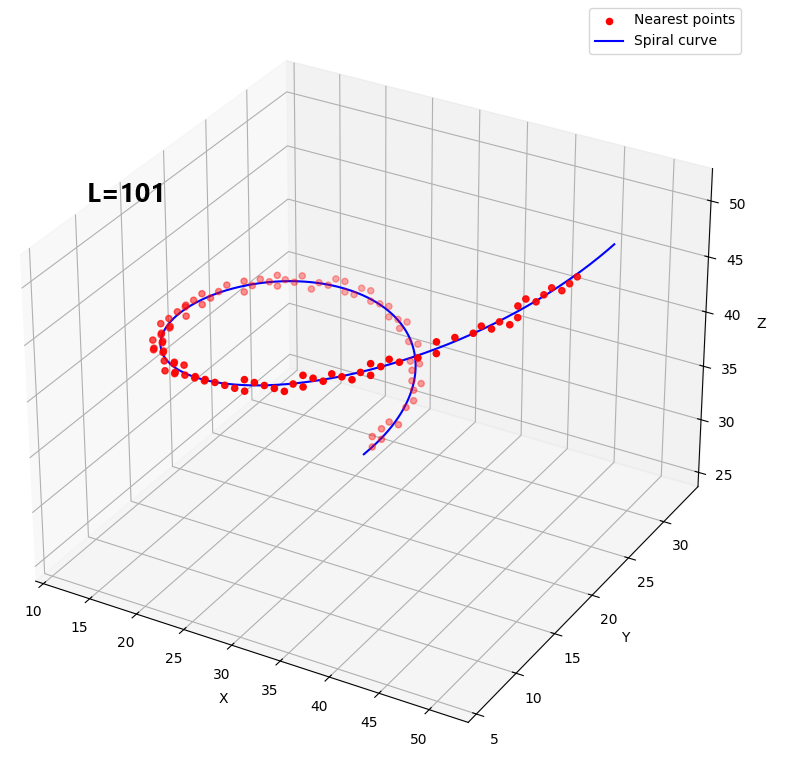
\includegraphics[width=10cm]{fig3}
\caption{The canonical spiral.}
\footnotesize{The canonical Archimedean spiral spans an angle of \(2\pi\) radians. It is replicated across each basis using a rotation matrix \( \mathbf{R} \). This path is the origin of light polarization patterns.}
\label{fig3}
\end{figure}

\subsection{Activating the pBit and sBit bits}
Vector $\hat{i}'_x$ is then used to mark the pBits from the center to the target point, following the well-known Bresenham 3D line algorithm. 

The points forming the spiral identify the cells that must have their $sB$ bit activated. These spiral patterns, parametrized across all layers, induce in particular the emergence of light polarization.

% ALGORITHMS
\newpage{}

\section{The convolution algorithm \label{sec:algorithms}}
Here are shown the convolution rules in two parts. Bubble $1$ is in the current lattice, while bubble $2$ is in the mirror lattice. Changes to bubble $1$ and bubble $2$ are made in the corresponding draft cell. More details beyond those shown here can be found in the text.

\begin{algorithm}
    \caption{Convolution algorithm - Part 1}
    \label{algo:convolution1}
    \begin{algorithmic}[1]
        \If{$T1=D1$ \textbf{and} $T2=D2$}
            \State $\triangleright$ Wavefronts active 
            \If{$X1=X2$}
                \State $\triangleright$ Superposition
                \If{$CH1=\sim CH2$ \textbf{and} $T1>0$ \textbf{and} $T1=T2$}
                    \State $\triangleright$ Segregation
                    \If{$pB1$}
                        \State $c1'=c1$
                    \EndIf   
                    \If{$pB2$}
                        \State $c2'=c2$
                    \EndIf   
                \ElsIf{$F1 = 1$ \textbf{and} $F2 = 1$}
                    \State $\triangleright$ Legal pair?
                    \If{$(CH1 \oplus CH2) \land W1M$}
                        \State $A1'=A2'=\min(A1, A2)$
                        \State $F1'=F2'=2$
                    \EndIf   
                \ElsIf{$F1 > 1$ \textbf{and} $F2 > 1$}
                    \State $\triangleright$ Multi-pair is legal?
                    \If{$CH1=CH2$}
                        \State $A1'=A2'=\min(A1, A2)$
                        \State $F1'=F2'=F1+F2$
                    \EndIf   
                \EndIf   
            \Else
                \State $\triangleright$ Distinct case
                \State (see Algorithm \ref{algo:convolution2})
            \EndIf   
        \EndIf   
        \State  % Creates an empty line
        \State \textbf{Legend:}
        \State W1M is the w1 bit mask

    \end{algorithmic}
\end{algorithm}

\begin{algorithm}
    \caption{Convolution algorithm - Part 2}
    \label{algo:convolution2}
    \small
    \begin{algorithmic}[1]
        \If{$CH1=\sim CH2$} \Comment{fully symmetric charges?}
            \State $\triangleright$ Singularization
            \State $F1'=F2'=1$; $A1'=W1;\,A2'=W2$
            \State $c1'=c2'=c1$ \Comment{relocate}
        \ElsIf{$F1=1$ \textbf{and} $F2=1$} \Comment{singleton x singleton}
            \If{$CLR1=\sim CLR2$ \textbf{and}  $CLR1 \neq 000B$ \textbf{and}  $CLR1 \neq 111B$}
                \State $\triangleright$ Quark cohesion
                \State $A1'=A2'=\min(A1, A2)$
                \State $c1'=c2'=c1$  \Comment{relocate}
            \ElsIf{$pBit1$ \textbf{and} $pBit2$ \textbf{and} $(CH1 \oplus CH2) \land W1M$}
                \State $\triangleright$ Annihilation
                \State $F1'=F2'=1$; $A1'=W1;\,A2'=W2$; $kB1'=kB2'=1$
                \State $c1'=c2'=c1$  \Comment{relocate}
            \ElsIf{($pBit1$ \textbf{or} $sBit1$) \textbf{and} ($pBit2$ \textbf{or} $sBit2$)}
                \If{lepton x lepton}
                    \State $\triangleright$ Lepton Cohesion
                    \State $A1'=A2'=\min(A1, A2)$
                    \State $c1'=c2'=c1$  \Comment{relocate}
                \ElsIf{lepton x lepton track}    
                    \State $\triangleright$ Lepton self-interference
                    \State $c1'=c2'=c1$  \Comment{relocate}
                \EndIf    
            \ElsIf{$pBit1$ \textbf{and} $pBit2$}
                \State $\triangleright$ Coulomb force
                \State $c1'=c2'=c1$  \Comment{relocate}
            \ElsIf{$sBit1$ \textbf{and} $sBit2$}
                \State $\triangleright$ Magnetism
                \State $c1'=c2'=c1$  \Comment{relocate}
            \EndIf   
        \ElsIf{$F1=1$ \textbf{and} $F2>1$ \textbf{and} $W1=W2$} \Comment{singleton x blob}
            \If{$CLR1=\sim CLR2$ \textbf{and}  $CLR1 \neq 000B$ \textbf{and}  $CLR1 \neq 111B$}
                \State $\triangleright$ Quark x gluon
                \State $c1'=c2'=c1$  \Comment{relocate}
            \ElsIf{$\phi B1$ \textbf{and} $\phi B2$ \textbf{and} $A1\neq W$}
                \If{E.M. interaction}
                    \State $\triangleright$ Light-matter interaction
                    \State $kB1'=kB2'=1$
                    \State $c1'=c2'=c1$  \Comment{relocate}
                \ElsIf{Weak interaction}
                    \State $\triangleright$ Fermion x weak boson OR fermion x neutrino
                    \State $c1'=c2'=c1$  \Comment{relocate}
                \EndIf        
            \EndIf   
        \ElsIf{$F1>1$ \textbf{and} $F2>1$} \Comment{both are blobs}
            \If{Strong interaction}
                \State $\triangleright$ Gluon x gluon
                \State $A1'=A2'=\min(A1, A2)$
                \State $c1'=c2'=c1$  \Comment{relocate}
            \ElsIf{Weak}
                \State $\triangleright$ Weak boson cohesion
                \State $A1'=A2'=\min(A1, A2)$
                \State $c1'=c2'=c1$  \Comment{relocate}
            \EndIf   
        \EndIf   
    \end{algorithmic}
\end{algorithm}

\end{document}
